\documentclass[12pt]{article}

\usepackage{amssymb,amsthm,amsmath}
\usepackage{mathtools} 
\usepackage{graphicx}
\usepackage{geometry,lscape}
\usepackage{longtable,multirow}
\usepackage{booktabs}
\usepackage{bbold}
\usepackage{tikz}
\usepackage[font={small,bf}]{caption}
\usepackage[title]{appendix}
\usepackage{dcolumn}
\usepackage{hyperref}
\newcolumntype{d}[1]{D{.}{.}{#1}}

\linepenalty=10
\captionsetup[table]{skip=5pt}
\geometry{a4paper}

\newtheorem{assumption}{Assumption}
\newtheorem{proposition}{Proposition}








\date{}
\author{Rong Fan}

\begin{document}

\begin{titlepage}
\title{Growth Model with Automation and Endogenous Human Capital}
\author{Rong Fan\thanks{I thank Bulent Guler, Todd Walker and Rupla Kamdar for their thorough guidance with this project.} 
\\
\\
\\ \href{https://rfan1994.github.io/files/Growth\%20Model.pdf}{https://rfan1994.github.io/files/Growth\%20Model.pdf}
\\ \href{https://rfan1994.github.io/files/Growth\%20Model.pdf}{Click here for newest version}}
\date{\today}
\maketitle

\begin{abstract}
\noindent Human capital accumulation responds to technological changes. I study the effects of automation industrial revolution on labor share, wage premium, and inequality under the framework of task model with heterogeneous workers (skilled and unskilled) and endogenous human capital. First, human capital accumulation races with automation, decreasing the automation level and increasing the labor share. Second, uneven responses of skilled and unskilled workers amplify the inequality effect, explaining 60\% of the wage premium increase. I calibrate the model by fitting the transition path to the data and discuss the policy to optimize the transition. Empirical evidence is provided at both industry and occupation levels. Automation has a positive effect on labor composition and overall skill level. The responses of skilled and unskilled workers are significantly different. \\
\vspace{0in}\\
\noindent\textbf{Keywords:} growth, technology, automation, inequality\\
\vspace{0in}\\
\noindent\textbf{JEL Classification: } J24, J31, O11, O14\\

\bigskip
\end{abstract}
\setcounter{page}{0}
\thispagestyle{empty}
\end{titlepage}
\pagebreak \newpage

\section{Introduction}
As has been argued in the literature, automation and artificial intelligence (AI) are essential in explaining the decrease in labor share (e.g., Autor and Salomons, 2018\cite{AutorSalomons2018}; Aghion et al., 2021\nocite{Aghionetal2021}) accompanied by the increase in college premium (e.g., Acemoglu and Autor, 2011\nocite{AcemogluAutor2011}; Acemoglu and Restrepo, 2020\nocite{AcemogluRestrepo2020}). Automation allows the machine to replace unskilled workers (high school graduates), decreasing the labor share while it complements skilled workers (college graduates), increasing the college premium.

Human capital accumulation is a vital response channel of workers to automation that has not been discussed much in the literature. Workers can respond to automation by increasing the supply of skilled workers (extensive margin). The share of employment with a Bachelor's degree and higher has increased from 26.98\% to 43.74\% from 1992 to 2021.\footnote{Data source: FRED (Federal Reserve Economic Data)} Additionally, workers can increase their skill level through on-the-job training (intensive margin). The ratio between training (e.g., GED, ESL, work related courses) and working hours has increased from 0.244\% to 1.049\% for high school graduates and from 0.758\% to 1.212\% for college graduates from 1995 to 2005.\footnote{Data source: ATES (Adult Training and Education Survey)} Acquisition of new skills can help unskilled workers to relocate to less automated sectors and help skilled workers to stand out in a more competitive labor market environment. 

Important questions are how the human capital of each skill group responds to automation and to what extent the response of human capital changes the effect of automation on the labor market (labor share and wage premium) and welfare inequality. Sachs and Kotlikoff (2012)\nocite{SachsKotlikoff2012} provide an earlier related study, which shows that young, low-skill workers respond to automation by decreasing investment in education because the wage depreciation limits their ability to save. Prettner and Strulik (2020)\nocite{PrettnerStrulik2020} show that automation increases the share of skilled workers because workers are motivated by higher wage premiums. In contrast to the existing studies on automation and human capital, I focus on after-school human capital accumulation. Athreya and Eberly (2015)\nocite{AthreyaEberly2015} discusses the stagnated college attainment accompanied by a substantial increase in the college premium. Not everyone is able or willing to attend college due to credit constraints or uncertainty, but most people spend a lot of time acquiring human capital throughout their life.

To study the interaction between automation and human capital and their macroeconomic implication, I adopt the task model framework of Acemoglu and Restrepo (2018)\nocite{AcemogluRestrepo2018}. Tasks are defined as units of work activity that produce output; they can be produced by machine (if automated) or labor. In section 2, I set up the model by introducing heterogeneous workers, endogenous human capital responses, and research and development (R\&D) sector to the basic task model. Workers are different in their skill levels (skilled and unskilled), skilled workers have comparative advantage over newer tasks and have a higher ability to adjust their human capital. I endogenize the human capital following Grossman et al.(2021)\nocite{Grossmanetal2021}. Human capital is accumulated by learning at the opportunity cost of wage income, but increases the productivity of workers. Research and development (R\&D) is directed and endogenous, skilled workers can become scientists and work in automation (automate old tasks favoring machine) or innovation (innovate new tasks favoring labor) sectors. 

I start by studying the effects of automation and human capital in a static model. Automation directly replaces unskilled workers (displacement effect), and indirectly affects skilled workers since unskilled workers relocate after being displaced (relocation effect). Accumulation of human capital increases the effective labor supply, pushes back automation and increases labor share. 

The direct effect is only a part of the story. In section 3, I embed this framework in a dynamic environment where I allow physical and human capital accumulation, and directed and endogenous R\&D. The increase of automation is endogenous, being a result of technological revolution -- a reduction in automation cost. After a reduction in automation cost, more scientists work in the automation sector and the automation level rises. This automation level increase is followed by increases of  innovation rate and human capital investment. A higher automation level complements the innovation sector since it drives up the capital price, pushes down the wage level, and increases the innovation patent profit. The development of innovation patents complements human capital investment, since it increases the future wage growth of workers. 

I highlight the uneven impacts of automation on skilled and unskilled workers and the distinctive responses of skilled and unskilled workers to automation. First, skilled workers benefit more from the productivity effect (improvement of allocation and higher innovation rate) of the technological revolution, while unskilled workers are affected more by the displacement effect. As a result, skilled workers increase their human capital investment more than unskilled workers. Skilled workers are more incentivized to invest in their human capital to maximize the benefit of automation. Unskilled workers save more through physical capital and less through human capital to insure against the wage drop caused by automation. Second, skilled and unskilled workers accumulate their human capital in different ways. Skilled workers acquire skills through learning-or-doing, making it easier to adjust their human capital in response to the technology change. On the other hand, unskilled workers accumulate human capital passively through learning-by-doing, adapting to the technology change more slowly.  

Before moving to section 5, where I implement counterfactual policy experiment, I solve the social planner's problem in section 4. There exist two externalities in the decentralized economy. First, skilled workers overinvest in their human capital. Skilled workers don't internalize their negative externalities in the R\&D sector. The opportunity cost of research is higher when skilled workers are more productive in the production sector. Second, too many tasks are automated. When developing innovation patents, the R\&D sector does not internalize the positive externalities they generate on existing tasks. Keeping that in mind, automation tax and training tax on skilled workers seem to be appropriate for the redistributive fiscal policy. 

In section 5, I calibrate the model, solve the transition numerically with the calibrated model, and implement counterfactual policy experiments. I calibrate the model to match the key macroeconomic variables in 1980 (before technological revolution) and 2005 (after technological revolution). The technological revolution is captured by a reduction of automation cost. Then I simulate the transition numerically and implement counterfactual policy experiment with automation tax or training tax on skilled workers. 

My research delivers three key results. First, a reduction of automation level not only increases the automation rate, but also innovation rate. Lower automation cost increases the automation level and improves the allocation, innovation sector develops more new tasks because of the productivity gain. Workers increase their human capital investment in response to the higher growth rate of the economy. Second, human capital investment complements innovation but substitutes automation. Human capital investment increases the effective labor supply, slows capital deepening. It decreases the overall level of automation and increases the labor share. With a high enough human capital growth rate, the human capital supply is abundant, the economy will never converge to a balanced growth path (BGP) where all the tasks are automated. Third, only 40\% of the wage premium change can be explained by the direct effect of automation, the rest of the wage premium change is contributed by the human capital change. Unskilled workers are directly displaced by machine when the task is automated, relocate to the tasks that skilled workers have more comparative advantages over, so they have to accept a lower wage to compete with skilled workers. Skilled workers benefit more from automation and are more incentivized than unskilled workers to invest in their human capital; they also have higher ability of adjusting their human capital investment. As a result, human capital gap between skilled and unskilled workers increases, leading to a higher wage premium. 

I provide empirical evidences in section 6, using both industry and occupation level data. By using EU KLEMS (EU level analysis of capital, labor, energy, materials and service inputs) data, I find a positive response of education level to the development of automation, but with a four-year lag. Occupational level evidences are provided using O*NET (Occupational Information Network) and ATES (Adult Training and Education Survey). Skill levels grow faster in the occupations that are more exposed to the automation, contributed mainly by the skilled workers. Skill level growth or human capital investment is decreasing in the occupational automation exposure level but increasing in the workers' education level. Skilled and unskilled workers respond differently to automation, a higher exposure to automation increases the human capital investment of skilled workers more than that of unskilled workers. 

This paper makes four contributions to the literature. First, this paper is closely related to the study of effects of automation on labor share, employment, wage and inequality. My contribution is to explore the human capital responses to automation, and the interaction of human capital with labor market and social welfare. Acemoglu and Autor (2011)\nocite{AcemogluAutor2011} and Acemoglu and Restrepo (2018)\nocite{AcemogluRestrepo2018} developed theoretical frameworks to explore the displacement effect of automation. Many empirical studies support the theoretical prediction and show that automation is important in explaining the on-going change on the US labor market. Autor and Salomons (2018)\nocite{AutorSalomons2018} use industry data and Dinlersoz et al.(2018)\nocite{Dinlersozetal2018} use plant based data to study the negative impact of automation on labor share. Robotization also reduces aggregate employment at the employment zone level (Aghioen et al., 2021\nocite{Aghioenetal2021}). In terms of inequality, automation can explain between 50\% and 70\% of changes in the US wage structure (Acemoglu and Restrepo, 2020\nocite{AcemogluRestrepo2020}) and increases the welfare inequality through return to wealth (Moll et al., 2021\nocite{Molletal2021}).

Second, my research contributes to the literature on endogenous growth\footnote{Aghion et al.(2014)\nocite{Aghionetal2014} survey Schumpeterian growth theory, in which new innovations replace older technologies, resulting in endogenous growth, individuals can choose to allocate the labor supply between production and research.} and technology adoption. The setup of research and development sector is similar to Acemoglu et al.(2013)\nocite{Acemogluetal2013}, unskilled workers are used in the production, while skilled workers perform R\&D functions and operations. In contrast to the canonical growth model, the research and development in my paper is directed, resources can be assigned to automation or innovation. Benhabib et al.(2017)\nocite{Benhabibetal2017} study how the adoption environment can change the innovation incentives and the growth rate. In this paper, the willingness of adoption of producers affects both the automation level and the growth rate. 

Third, this paper contributes to the literature on human capital accumulation. I explore the heterogeneous human capital investment for different skill groups facing increasing automation. The accumulation of human capital takes two forms. First, knowledge is passed across generations through education, the initial skill type of the workers is determined by their choice schooling investment. (Schultz, 2003\nocite{Schultz2003}; Bohacek and Kapicka, 2008\nocite{BohacekKapicka2008}) Second, human capital can be increased through learning-by-doing (experience will be accumulated by doing the job, e.g., Imai et al., 2004\nocite{Imaietal2004}; Thompson, 2010\nocite{Thompson2010}; Burdett et al., 2011\nocite{Burdettetal2011}) or learning-or-doing (workers need to spend time to learn new skills with the opportunity cost of production, e.g., Frazis, 2007\nocite{Frazis2007}). This paper focuses mainly on after-school human capital acquisition following Stantcheva, 2015\nocite{Stantcheva2015}, the agents optimally choose working and training time, human capital evolves depending on the amount of training, and individuals are heterogeneous in terms of their ability. 

Last, my paper explores the interaction between human capital and technology, but distinguishes automation (replaces labor) and innovation (complements labor) as two types of technological change. Technology and human capital can be twin engines of the growth, but can also be opponents racing against each other. The dynamics between innovation and human capital in this paper are similar with Lloyd-Ellis and Roberts (2002)\nocite{Lloyd-EllisRoberts2002}, skills are required to implement and invent new technology; Beaudry et al.(2006)\nocite{Beaudryetal2006}, new technology is more productive and will be adopted only when used with a high fraction of skill workers; and Stokey (2014)\nocite{Stokey2014} and Stokey (2020)\nocite{Stokey2020}, the endogenous growth would happen only if both parts grow at the same time. However, the relationship between automation technology and human capital are competitive. Since workers and R\&D sectors are making decisions separately, growth can be described as a strategic game between workers and entrepreneurs on decisions of human capital and R\&D investment as described in Redding (1996)\nocite{Redding1996}.


\section{Model with Automation}
In this part of the paper, I develop a growth model with endogenous innovation, automation and human capital. I adopt the framework of task model developed by Acemoglu and Restrepo (2018)\nocite{AcemogluRestrepo2018}. However, I focus on the directed research and development investment and the endogenous human capital investment. The human capital growth is endogenized following Grossman et al.(2021)\nocite{Grossmanetal2021}, but with more generalized accumulation functions. 

\subsection{Environment}
Figure \ref{model} presents the structure of the model. The formal model of the economy has three sectors: household, production, and the research and development (R\&D) sector. There are two types of households: unskilled and skilled. Households consume, save and invest in human capital. Final good producers produce consumption goods by combining tasks produced by task producers. Tasks are defined as units of work activity that produce output. To produce tasks, task producers purchase patent intermediates (innovation or automation) from the R\&D sector and combine them with production factors (capital, low-skill or high-skill labor). Unskilled workers can only work in the production sector, supplying low-skill labor. Skilled workers can work both in the production and the R\&D sector, supplying high-skill labor or working as scientists to develop innovation or automation patents. 

\begin{figure}[h!]
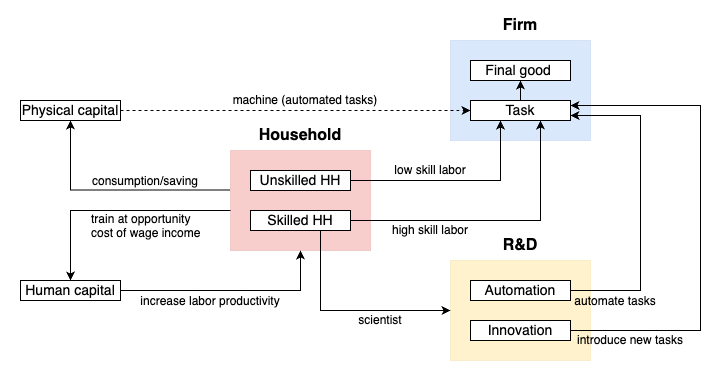
\includegraphics[width = \textwidth]{Model}
\caption{Model Structure}
\label{model}
\end{figure}

The economy is populated by two types of representative households: skilled households and unskilled households. They have the same preference and discount rate, but supply different types of labor and have different learning abilities. The households make two decisions simultaneously. First, they make consumption-saving decisions to maximize lifetime utility. Second, they allocate their time between working and training to optimize their lifetime wage income. Unskilled households supply low-skill labor, and skilled household supply high-skill labor or work as scientists. Physical and human capital are two alternative ways for households to save for the future. If the return to physical capital (interest rate) is higher, households will prefer to save through physical capital; if the return to human capital (wage growth rate) is higher, they will favor human capital investment. 

There are task and final good producers in the production sector, and all the producers are perfectly competitive. To produce tasks, task producers purchase patent intermediates from the R\&D sector and combine them with production factors. If the task has been automated, the producers of this task will purchase automation patent intermediates and choose between labor (low and high-skill) and machines to minimize the production cost. If the task hasn't been automated, the producers of this task will purchase innovation patent intermediates and can only choose between low and high-skill labor to produce the intermediate goods. The final good producers purchase the tasks from the task producers at competitive prices and use a CES production function to combine them into the consumption goods. 

The skilled workers can work as scientists in the R\&D sector to develop new patents. There are two types of patents: innovation patents bring new tasks to the economy, which increases labor productivity and can only be produced by labor; automaton patents allow the firm to use capital instead of labor to produce the task. After developing the patent, the scientists hold the patent right and sell the task-specific patent intermediates to task producers at the price $\psi$. The growth of the economy is endogenous and Schumpeterian. The old tasks are destroyed when new ones are introduced, keeping the task measure constant.\footnote{The task productivity is increasing in the task index. If the variety growth is not excluded, the growth rate will increase over time and converge to infinity.} 

\subsubsection*{Household}
The economy is populated by two types of representative households: skilled households with measure $\epsilon_H$ and unskilled households with measure $\epsilon_L$. They share the same CRRA preference $\frac{C^{1-\theta}}{1-\theta}$, with $\theta$ being the intertemporal elasticity of substitution, and discount rate $\rho$. However, they supply different types of labor and have different leaning abilities. Households maximize their lifetime utility by making consumption-saving and working-learning decisions. 

Unskilled households can only work in production sector and supply low-skill labor. Each period, they receive return to capital $K_L$ at rate $r$, wage income $W_L$, and transfer from the government $T_L$. Given the current technological environment, they allocate their time $l_L$ to working and $1-l_L$ to training. The total low-skill labor supply is $\epsilon_Ll_L$. By allocating time to learning, they can increase the wage by increasing their human capital, but at the opportunity cost of wage income. The accumulation of human capital is increasing in the time spent on training. Unskilled households maximize their lifetime utility: 
\begin{align*}
\rho V_L(K_L,h_L) = \max_{C_L,L_L,1-l_L} \quad \frac{C_L^{1-\theta}}{1-\theta}+V_{LK}(K_L,h_L)\dot{K}_L+V_{Lh}(K_L,h_L)\dot{h}_L,
\end{align*}
subject to the laws of motion of physical and human capital: 
\begin{align*}
\dot{K}_L &=r K_L+\frac{W_LL_L}{\epsilon_L}-\tau_{hL}W_L(1-l_L)+T_L-C_L, \\
\dot{h}_L &= \frac{(1-l_L)^{\alpha_L}}{\mu_{hL}}, \\
L_L &=\epsilon_L l_L.
\end{align*}

Skilled households also receive the return to capital $K_H$ at rate$r$, and transfer from the government $T_H$. They are different from unskilled workers in that they can work in the production sector by supplying high-skill labor $L_H$ or the R\&D sector by supplying research labor for automation ($\epsilon_I$) and innovation ($\epsilon_N$). When they work in the production sector, they receive the wage income $W_H$. When they work in the research sector, they hold the patent they develop and receive the patent profits $\Pi$ by selling patent intermediates to task producers. Skilled households maximize their lifetime utility: 
\begin{align*}
\rho V_H(K_H,h_H) = \max_{C_H,L_H,1-l_H} \quad \frac{C_H^{1-\theta}}{1-\theta}+V_{HK}(K_H,h_H)\dot{K}_H+V_{Hh}(K_H,h_H)\dot{h}_H,
\end{align*}
subject to the low of motion of physical and human capital: 
\begin{align*}
\dot{K}_H &= r_t K_H +\frac{W_H L_H+\Pi}{\epsilon_H}-\tau_{hH}W_H(1-l_H)+T_H-C_H, \\
\dot{h}_H &= \frac{(1-l_H)^{\alpha_H}}{\mu_{hH}}, \\
 L_H&=\epsilon_H l_H-\epsilon_N-\epsilon_I.
\end{align*}
Government subsidizes training at rates $\tau_{hL}$ and $\tau_{hH}$ for unskilled and skilled workers. Training subsidy is linear in the opportunity cost of training. 

The law of motion for human capital is a generalized form of Grossman et al.(2021)\nocite{Grossmanetal2021}. $\mu_{hL}$ and $\mu_{hH}$ capture the training efficiency, and $\alpha_L$ and $\alpha_H$ represent the training style. The training efficiency is decreasing in $\mu_{hj}, j\in\{L,H\}$, and the human capital growth converges to 0 when $\mu_{hj}$ converges to infinity. When $\alpha_j \to 0$, the human capital is accumulated through learning-by-doing, and the human capital growth rate is constant, no matter how much time the workers spend on training. When $\alpha_j \to 1$, the human capital is accumulated through learning-or-doing, and the human capital accumulation rate is linear in the time spent on training.\footnote{Grossman et al.(2021) is a special case: $\mu = 1$ and $\alpha=1$}. Here I assume that $0\leq\alpha_L<\alpha_H\leq1$, skilled workers can adjust their human capital accumulation more easily through on-the-job training than unskilled workers, and unskilled workers mainly accumulate their human capital passively through working experience. 

\subsubsection*{Production Sector}

The final good sector is perfectly competitive and produce the consumption good $Y$ by combining a unit measure of tasks $i\in [N-1,N]$, with an elasticity of substitution $\sigma \in (0,\infty)$. $y(i)$ is the output of each task $i$. The creation of newest tasks will destroy the oldest tasks, so the total measure of the task in this economy remains constant $1$. The production function of final good sector takes the form:
\begin{align*}
Y = \tilde{A}\Big(\int_{N-1}^{N}y(i)^{\frac{\sigma-1}{\sigma}}di\Big)^{\frac{\sigma}{\sigma-1}}.
\end{align*}
The competitive final good producers purchase the task $i$ from task producer at price $p(i)$, and solve the following problem:
\begin{align*}
\max \quad & Y-\int_{N-1}^Np(i)y(i)di. 
\end{align*}

The task sector is also competitive; task producers purchase task-specific intermediates $q(i)$ at price $\psi$ from patent holders, which embodies the technology. Then they combine the task-specific intermediates with production factors (capital or labor). Suppose the automation patent has not been developed for the task. In that case, the task producers can only purchase the innovation patent intermediates. They can only use labor (high-skill $h(i)$ or low-skill $l(i)$) to produce the intermediate goods $y(i)$. If the task has been automated, the task producer can choose between automation and innovation patent and combine capital $k(i)$ with automation patent or labor with innovation patent. The production function of task producers is Cobb-Douglass:
\begin{align*}
y(i) &= 
\begin{dcases}
q(i)^{\eta}\Big(k(i) + \gamma_L(i,h_L)l(i)+\gamma_H(i,h_H)h(i)\Big)^{1-\eta} , &\quad \text{$i$ is automated}  \\
q(i)^{\eta}\Big(\gamma_L(i,h_L)l(i)+\gamma_H(i,h_H)h(i)\Big)^{1-\eta} ,&\quad \text{$i$ is not automated}
\end{dcases}. 
\end{align*}
When the intermediate goods $y(i)$ are produced with machine, the productivity is normalized to 1. The productivity of the skilled worker $\gamma_H(i,h_H)$ and the unskilled worker $\gamma_L(i,h_L)$ is increasing in the task index $i$ and the worker's human capital level $h_H$ and $h_L$. 
The task producers solve the following problem:
\begin{align*}
\max \quad  p(i)&y(i)-Rk(i)-W_Ll(i)-W_Hh(i)-\psi q(i).
\end{align*}

\subsubsection*{Research Sector}
Some skilled workers will work as scientists in the R\&D sector to develop new automation and innovation patents. An innovation patent introduces a new task to the economy and increases the productivity of labor, automation patent allows the firm to produce the task using machines and improves the production factor allocation. After developing new patents, they sell task-specific intermediates to task producers at the price $\psi$ until the patent is outdated and destroyed. When the patent is destroyed, the patent will be forced to exit the market and get compensated by the new entry. \footnote{I borrow this structure of intellectual property rights from Acemoglu and Restrepo(2018)\nocite{AcemogluRestrepo2018} to remove the creative destruction. They show that the structure with creative destruction has similar implications but introduces additional unstability to the model.} The values of automation and innovation patents are defined as the sum of discounted profit by selling patent intermediates, denoted by $P_N$ and $P_I$. The amount of automation and innovation patents introduced to the economy ($\kappa_I$ and $\kappa_N$) are functions of scientists hired in each sector ($\epsilon_I$ and $\epsilon_N$).
Assume that the production functions of the R\&D sector take the form: 
\begin{align}
\label{kappa_I}
\kappa_I(\epsilon_I) &= \frac{\epsilon_I^\lambda}{\mu_I}, \\
\label{kappa_N}
\kappa_N(\epsilon_N) &= \frac{\epsilon_N^\lambda}{\mu_N}, \quad 0<\lambda\leq 1.
\end{align}

The amount of new patents developed is increasing in the scientists working in the sector, with decreasing marginal productivity. Bloom et al.(2020)\nocite{Bloometal2020} find empirical evidence showing that research effort is rising while research productivity is declining. $\mu_I$ and $\mu_N$ capture the research efficiency. The research is more efficient with smaller $\mu_I$ and $\mu_N$. 

\subsection{Static Model Equilibrium}
In this subsection, I start with a static version of the model to characterize the impact of automation, innovation and human capital on allocation, factor prices and labor share. In section 3, I bring the static framework to a dynamic environment, to understand the interaction between the change of technology and human capital. 

By solving the final good producers' problem (see appendix), we can derive the demand function for task $i$ as a function of the task price:
\begin{align*}
y(i) = \tilde{A}^{\sigma-1}Yp(i)^{-\sigma}.
\end{align*}

The task producers sell the tasks to final good producers. The task sector is perfectly competitive, so the price of the task $p(i)$ will equal the cost of production (see appendix). The effective cost depends on the ratio between the factor price and the factor productivity of the task. When the task has been automated, the task producers will choose between capital and labor to minimize the production cost; when the task is new and has not been automated, the task producers can only select between high-skill and low-skill labor. The task price of task $i$ can be written as: 
\begin{align*}
p(i) &= 
\begin{dcases}
\Psi \min\{R^{1-\eta},\Big(\frac{W_L}{\gamma_L(i,h_L)}\Big)^{1-\eta},\Big(\frac{W_H}{\gamma_L(i,h_H)}\Big)^{1-\eta}\} &\text{, if automated}  \\
\Psi \min\{\Big(\frac{W_L}{\gamma_L(i,h_L)}\Big)^{1-\eta},\Big(\frac{W_H}{\gamma_L(i,h_H)}\Big)^{1-\eta}\} &\text{, if new,}
\end{dcases}
\end{align*}
where $\Psi = (\frac{\psi}{\eta})^{\eta}(\frac{1}{1-\eta})^{1-\eta}$. 

Plug the price $p(i)$ in the demand function derived from the final good sector above, the output of each task can be solved as (see Appendix): 
\begin{align*}
p(i)y(i) &= 
\begin{dcases}
Y\Big(\frac{R}{A}\Big)^{1-\hat{\sigma}}, &\quad  \text{, using capital}  \\
Y\Big(\frac{W_L}{A\gamma_L(i,h_L)}\Big)^{1-\hat{\sigma}}, &\quad  \text{, using low-skill labor}    \\
Y\Big(\frac{W_H}{A\gamma_H(i,h_H)}\Big)^{1-\hat{\sigma}}, &\quad  \text{, using high-skill labor}, 
\end{dcases}
\end{align*}
where $\hat{\sigma} = 1-(1-\eta)(1-\sigma)$ and $A = \Big(\frac{\tilde{A}}{\Psi}\Big)^{\frac{\sigma-1}{\hat{\sigma}-1}}  = \Big(\frac{\tilde{A}}{\Psi}\Big)^{\frac{1}{1-\eta}}$.

\begin{assumption}{\bf (Elasticity of Substitution)} \\

Assume that $\hat{\sigma}>1$
\end{assumption}

When $\hat{\sigma}>1$, the tasks are substitutes. The output of the task is increasing in the task productivity and decreasing in the factor price. The demands for factors are decreasing in the factor prices. More workers are hired when they have higher task productivity. 


\begin{assumption}{\bf (Task Productivity)} \\

Assume that skilled workers have comparative advantage in high index tasks over machine and unskilled workers, all workers have absolute advantage over machine. The productivity of machine is constant over all tasks and is normalized to 1. 
\begin{align*}
\gamma_K &= 1 \\
\gamma_H(i,h_H) &=e^{B(i)} e^{bh_H} \\
\gamma_L(i,h_L) &= e^{B(N-1)+B_L(i-(N-1))} e^{bh_L}
\end{align*}
\end{assumption}

The innovation patent is complementary to skill and directly increases the productivity of skilled workers at the rate $B$. The technology also has a spillover effect and increases the productivity of unskilled workers.\footnote{To assure the existence of a balanced growth path. Without the spillover effect, the wage premium $W_H/W_L$ converges to infinity in the long run.} The productivity of skilled and unskilled workers is always the same for the most outdated task ($N-1$), but skilled workers have a comparative advantage over unskilled workers for new tasks. The newer the tasks, the more comparative advantage the skilled workers have. Task productivity is also increasing in the human capital level. Human capital is general and increases workers' productivity for all tasks.  


\begin{proposition}{\bf (Allocation)} \\

Research sector always automate from the low index tasks, there exists automation level $I$, such that all the tasks between $N-1$ and $I$ are produced by machine, and all the tasks between $I$ and $N$ are produced by labor. Given automation level $I$, there exists cutoff point $S$, such that all the tasks between $I$ and $S$ are produced by high-skill labor, and all the tasks between $S$ and $N$ are produced by low-skill labor. 

The task producers have incentive to adopt the newest automation patent when the following condition is satisfied:
\begin{align*}
R < \frac{W_L}{\gamma_L(I,h_L)}
\end{align*}
The task producers have incentive to adopt the newest innovation patent when the following condition is satisfied: 
\begin{align*}
R > \frac{W_H}{\gamma_H(N,h_H)}
\end{align*}
The allocation $S$ must satisfy the non-arbitrage condition: 
\begin{align*}
\frac{W_H}{\gamma_H(S,h_L)} = \frac{W_L}{\gamma_L(S,h_L)}
\end{align*}
\end{proposition}
\noindent{\bf Proof.} See Appendix B.

\begin{figure}[h!]
\center
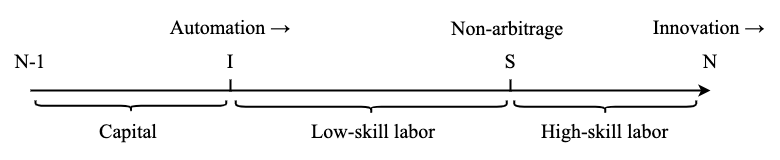
\includegraphics[width=0.8\textwidth]{allocation}
\caption{Task Allocation}
\label{allocation}
\end{figure}
Figure \ref{allocation} presents the task allocation. Workers have comparative advantage over machine on more updated tasks. The R\&D sector will always automate the oldest tasks that have not been automated, because the automation patent can generate more profit in the more outdated tasks. The R\&D sector have incentive to develop the automation patent only if the firm is willing to purchase the automation patent once the patent is developed; so all the automated tasks are produced using machine. For the tasks that are not automated, skilled workers have more advantage in the high index tasks, so the newest tasks are taken by skilled workers, and the unskilled workers will take the less updated tasks. 


\begin{proposition}{\bf (Equilibrium in Static Model)} \\

After solving the firm's optimization problem, and applying market clearing condition, the aggregate production function can be written as CES production function, where the productivity of each production factor is determined endogenously by allocation: 
\begin{align}
\label{output}
Y = \frac{A}{1-\eta}\Big((\Gamma_KK)^{\frac{\hat{\sigma}-1}{\hat{\sigma}}}+(\Gamma_LL_L)^{\frac{\hat{\sigma}-1}{\hat{\sigma}}}+(\Gamma_HL_H)^{\frac{\hat{\sigma}-1}{\hat{\sigma}}}\Big)^{\frac{\hat{\sigma}}{\hat{\sigma}-1}}.
\end{align}
The equilibrium price and factor share can be solved similar to a standard CES production function: 
\begin{align*}
R &=A\Gamma_K\Big(\frac{(1-\eta)Y}{A\Gamma_KK}\Big)^{\frac{1}{\hat{\sigma}}},   \quad s_K= \frac{RK}{Y},  \\
W_H &=A\Gamma_H\Big(\frac{(1-\eta)Y}{A\Gamma_HL_H}\Big)^{\frac{1}{\hat{\sigma}}},  \quad s_H = \frac{W_HL_H}{Y},  \\
W_L &= A\Gamma_L\Big(\frac{(1-\eta)Y}{A\Gamma_LL_L}\Big)^{\frac{1}{\hat{\sigma}}},  \quad s_L = \frac{W_LL_L}{Y},   \\
\omega &= \frac{W_H}{W_L} = \Big(\frac{\Gamma_H}{\Gamma_L} \Big)^{\frac{\hat{\sigma}-1}{\hat{\sigma}}}\Big(\frac{L_L}{L_H} \Big)^{\frac{1}{\hat{\sigma}}}, 
\end{align*}
where $\Gamma_K$, $\Gamma_L$, and $\Gamma_H$ represent the productivity of capital, low-skill and high-skill labor, and are determined endogenously by allocation: 
\begin{align}
\label{Gamma_K}
\Gamma_K(\tilde{I}) &= \tilde{I}^{\frac{1}{\hat{\sigma}-1}}, \\
\label{Gamma_H}
\begin{split}
\Gamma_H(N,\tilde{I},\tilde{S},h_H)  &= \gamma_H(N,h_H)\Big(\frac{1-e^{-B(1-\tilde{S})(\hat{\sigma}-1)}}{B(\hat{\sigma}-1)}\Big)^{\frac{1}{\hat{\sigma}-1}} \\
&= \underbrace{\gamma_H(N,h_H)}_{\text{Tech frontier}}\underbrace{\tilde{\Gamma}_H(\tilde{S})}_{\text{Allocation}},
\end{split}
\\
\label{Gamma_L}
\begin{split}
\Gamma_L(N,\tilde{I},\tilde{S},h_L)  &= \gamma_L(N,h_L)\Big(\frac{e^{-B_L(1-\tilde{S})(\hat{\sigma}-1)}-e^{-B_L(1-\tilde{I})(\hat{\sigma}-1)}}{B_L(\hat{\sigma}-1)}\Big)^{\frac{1}{\hat{\sigma}-1}}\\
 &=\frac{\gamma_H(N,h_H)}{\gamma_{HL}}\tilde{\Gamma}_L(\tilde{I},\tilde{S}).
 \end{split}
\end{align}
And $\tilde{I} = I-(N-1)$ represents the automation level, and $\tilde{S} = S-(N-1)$ represents the labor allocation. $\gamma_{HL} = e^{(B-B_L)+bh_{HL}}$ represents the absolute advantage of skilled labor over unskilled labor on the frontier task $N$, $h_{HL} = h_H-h_L$ represents the human capital gap between skilled and unskilled workers.  
\end{proposition}

Figure \ref{allocation2} presents the change in task allocation after an increase of automation level. As shown in equation (\ref{Gamma_K}), capital productivity $\Gamma_K$ is a function of automation. When more tasks are automated, task producers use the machine to replace labor, $\Gamma_K$ increases, but $\Gamma_L$ and $\Gamma_H$ decreases. An increase in automation level increases the demand for capital but reduces the demand for both types of labor. As a result, the capital share increases, and the labor share decreases. Innovation does the opposite; it introduces new labor tasks, destroys old machine tasks, and increases labor productivity. 

As shown in equation (\ref{Gamma_H}) and (\ref{Gamma_L}), labor productivity $\Gamma_H$ and $\Gamma_L$ depend on the allocation and human capital level. Human capital accumulation increases $\Gamma_L$ and $\Gamma_H$, which raises the wage level and labor share. $\Gamma_H$ and $\Gamma_L$ can be decomposed into two parts. The first part, $\gamma_H(N,h_H)$ or $\gamma_L(N,h_L)$, represents the technology frontier, the highest task productivity of each skill group. The second part, $\tilde{\Gamma}_H$ or $\tilde{\Gamma}_L$, captures the allocation. i.e., the range of tasks produced by this type of worker. The ratio between $\Gamma_H$ and $\Gamma_L$ is increasing in the comparative advantage of skilled workers $B-B_L$ and the human capital gap $h_{HL}$. More tasks are produced by skilled workers when skilled workers have a higher comparative advantage and larger human capital gap than unskilled workers. The skill wage premium increases when more tasks are assigned to skilled workers. 

\begin{figure}[h!]
\center
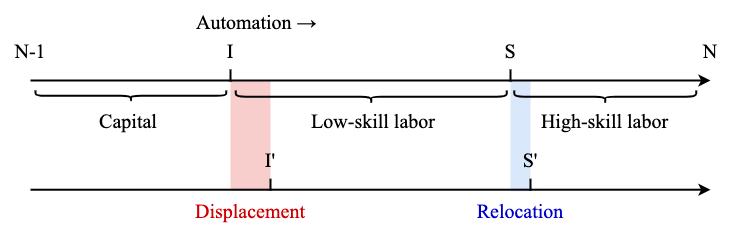
\includegraphics[width=0.8\textwidth]{allocation2}
\caption{Change in Task Allocation}
\label{allocation2}
\end{figure}


\begin{proposition}{\bf (Comparative Statistics)} \\
The change of labor share is given by the following equation: 
\begin{align}
\label{ds_L}
\begin{split}
d\ln(s_{L}+s_{H}) &= \frac{\hat{\sigma}-1}{\hat{\sigma}}\frac{s_K}{1-\eta}\underbrace{( \frac{s_L}{s_L+s_H}\frac{d\ln\tilde{\Gamma}_L}{d\tilde{I}}-\frac{d\ln H}{d\tilde{I}}}_{\text{Automation}})d\tilde{I}\\
&-\frac{\hat{\sigma}-1}{\hat{\sigma}}\frac{s_K}{1-\eta}\underbrace{(d\ln K -BdN-bdh-d\ln L)}_{\text{Capital deepening}},
 \end{split}
\end{align}
where the average change of human capital and labor supply is defined as: 
\begin{align*}
d\ln h &= \frac{s_H}{s_H+s_L}d\ln h_H+\frac{s_L}{s_H+s_L}d\ln h_L,\\
d\ln L &= \frac{s_H}{s_H+s_L}d\ln L_L+\frac{s_L}{s_H+s_L}d\ln L_L.
\end{align*}
The change of allocation $\tilde{S}$ and wage can be written as: 
\begin{align}
\label{dS}
\underbrace{d\tilde{S}}_{\text{Allocation}} &= \frac{1}{\epsilon(\tilde{S})}\Big(\underbrace{\frac{1}{\hat{\sigma}}(d\ln L_L-d\ln L_H-bdh_{HL})}_{\text{Labor supply}}-\underbrace{\frac{\hat{\sigma}-1}{\hat{\sigma}}\frac{d\ln\tilde{\Gamma}_L}{d\tilde{I}}d\tilde{I}}_{\text{Automaton}}\Big),\\ 
\label{dW_L}
d \ln W_L &= \underbrace{d \ln Y}_{\text{Productivity}} + \underbrace{\frac{\hat{\sigma}-1}{\hat{\sigma}}\frac{d\ln\tilde{\Gamma}_L}{d\tilde{I}}d\tilde{I}}_{Displacement}+ \underbrace{\frac{\hat{\sigma}-1}{\hat{\sigma}}\frac{d\ln\tilde{\Gamma}_L}{d\tilde{S}}d\tilde{S}}_{\text{Relocate}},\\
\label{dW_H}
d \ln W_H &= \underbrace{d \ln Y}_{\text{Productivity}}  + \underbrace{\frac{\hat{\sigma}-1}{\hat{\sigma}}\frac{d\ln\tilde{\Gamma}_H}{d\tilde{S}}d\tilde{S}}_{\text{Relocate}}, \\
\label{dw}
d \ln \omega &=(B-B_L)d\tilde{S}+bdh_{HL},
\end{align}
where $\epsilon(\tilde{S})$ is the inverse of allocation elasticity taking the form:  
\begin{align}
\label{eS}
\epsilon(\tilde{S})&= \underbrace{\frac{\hat{\sigma}-1}{\hat{\sigma}}(\frac{d\ln \tilde{\Gamma}_L}{d\tilde{S}}-\frac{d\ln \tilde{\Gamma}_H}{d\tilde{S}})}_{\text{Wage elasticity}}
								 +\underbrace{(B-B_L)}_{\text{Comparative advantage}}.
\end{align}
\end{proposition}

As shown in equation (\ref{dS}), right after an increase in automation, the wage of unskilled workers decreases through the displacement effect shown in equation  (\ref{dW_L}). At the original cutoff point $S$, the unit cost of using unskilled workers will be lower than using skilled workers. The unskilled workers then relocates and take on some tasks that used to be performed by skilled workers until the non-arbitrage condition is satisfied again. The shift of allocation $S$ depends on the allocation elasticity derived in equation (\ref{eS}). The labor allocation change is decreasing in the wage elasticity and comparative advantage of skilled workers. When the wage is elastic to the allocation, the non-arbitrage condition will be satisfied with a slight allocation change. With a high comparative advantage of skilled workers, the allocation will be sticky since it's difficult to use unskilled workers to substitute the skilled workers. 

Equation (\ref{ds_L}) shows how the labor share responds to the change in automation and human capital. An increase in automation decreases the labor share since it displaces unskilled workers directly. Human capital accumulation increases the labor share by increasing the effective labor supply. 

The responses of wage level are calculated in equation (\ref{dW_L}) and (\ref{dW_H}). Since automation improves the allocation, it increases the wage for all the workers through the productivity effect. However, it decreases the wage of unskilled workers directly through the displacement effect and the wage of skilled workers through relocation. 

After an increase in automation, the wage premium, as shown in equation (\ref{dw}), always increases. Automation pushes unskilled workers to tasks where they have a disadvantage compared to skilled workers. The change in wage premium is increasing in the comparative advantage and decreasing in the wage elasticity. When the comparative advantage is higher, the unskilled workers will absorb more impact from automation since the cost of relocation for unskilled workers is high. Unskilled workers will have to accept a lower wage to compete with skilled workers because their productivity is much lower at those tasks. When the wage elasticity is higher, the unskilled workers can pass more effects of automation to skilled workers since they can benefit more from the relocation.

Automation and human capital are two opposite forces determining labor share. An increase in automation decreases the labor share, while an increase in human capital does the opposite. Although unskilled workers can relocate after an increase in automation, an increase in automation always raise the wage premium. The wage premium increases more when the comparative advantage of skilled workers is high, and the wage is inelastic to the allocation. The total change of wage premium after an increase in automation also depends on the human capital response. If the human capital gap is enlarged after an increase in automation, the effect of automation on inequality will be amplified. In order to understand the full effect of automation, in the next section, I bring the static frame into a dynamic environment. 


\section{Dynamics and Balanced Growth Path}
In this section, I extend the static framework above into a dynamic environment. First, capital accumulation is endogenous. The capital accumulation responds to the change of technology and human capital growth. Second, the human capital growth is endogenous, depending on the time spent on training. Third, the R\&D is endogenous and directed, the automation level and technology growth rate is a result of R\&D investment.

\subsection{Balanced Growth Path}
\subsubsection*{Household}
Given the interest rate $r(t)$, wage $W_H(h_H,t)$ and $W_L(h_L,t)$, technology growth rate $g_N(t)$ and $g_I(t)$, and human capital growth rate $g_{hH}(t)$ and  $g_{hL}(t)$, households maximize their lifetime utility. By solving the households' problem, I can solve the intertemporal Euler equation, which characterizes the consumption-saving decision: 
\begin{align*}
\frac{\dot{C}_H}{C_H} &= \frac{\dot{C}_L}{C_L}  = \frac{r-\rho}{\theta} 
\end{align*}

The intratemporal Euler equation characterizes the optimal training decision for unskilled and skilled workers $j\in\{L,H\}$
\begin{align*}
&\underbrace{\frac{\delta \log W_j(h_j)l_j}{\delta h_j}\frac{\delta \dot{h}_j}{\delta (1-l_j)}}_{\text{Direct wage gain}}+\underbrace{\frac{\delta \log W_j(h_j)}{\delta h_j}\dot{h}_j+\frac{\delta \log W_j(h_j)}{\delta t}}_{\text{Return to human capital}}= r(1+\tau_{hj})
\end{align*}
The physical capital and the human capital are two ways for the workers to save for the future. The training incentive is decreasing in interest rate $r$, high interest rate increases the opportunity cost of training. The training incentive is increasing in the return to human capital. Higher wage growth makes the household more willing to put effort into the training.

By plugging in the production function, marginal return rate of training is constant $b$, since the human capital is general and the growth rate of wage is linear in the human capital increase. 
\begin{align*}
\frac{d\log W_H(h_H,t)}{dh_H} = \frac{d\log W_L(h_L,t)}{dh_L} = b
\end{align*}
Equation (\ref{gW_H}) and (\ref{gW_L}) characterize the wage growth rates of skilled and unskilled workers. They depend mainly on the technology and human capital growth rate. The growth rate of physical capital and labor supply also has an impact on the wage growth rate. 
\begin{align}
\label{gW_H}
\frac{dW_H(h_H,t)}{dt} &= g_{WN}+g_{WI}+\frac{s_L}{s_H+s_L}g_{WS}\\
\label{gW_L}
\frac{dW_L(h_L,t)}{dt}  &= g_{WN}+g_{WI}-\frac{s_H}{s_H+s_L}g_{WS}
\end{align}
I decompose the wage growth into three components. $g_{WN}$ and $g_{WI}$ are common effect of innovation and automation on wage growth for both skilled and unskilled workers.The difference between the skilled and unskilled workers' wage growth is contributed mainly by the shift of allocation $g_{WS}$:  
\begin{align}
\label{g_WN}
g_{WN} &= \underbrace{Bg_N}_{\text{Productivity}}+\underbrace{a(\tilde{I})(g_K-g_L-Bg_N-bg_h)}_{\text{Capital deepening}}, \\
\label{g_WI}
g_{WI} &= \underbrace{a(\tilde{I})\frac{d\ln H}{d\tilde{I}}(g_I-g_N)}_{\text{Productivity}}+\underbrace{\frac{s_L}{s_H+s_L}(1-a(\tilde{I}))\frac{d\ln \tilde{\Gamma}_L}{d\tilde{I}}(g_I-g_N)}_{\text{Displacement}}, \\
\label{g_WS}
g_{WS}&= \frac{B-B_L}{\epsilon(\tilde{S})}(\underbrace{\frac{1}{\hat{\sigma}}(g_{LL}-g_{LH}+b(g_{hL}-g_{hH}))}_{\text{Labor supply}}-\underbrace{\frac{\hat{\sigma}-1}{\hat{\sigma}}\frac{d\ln \tilde{\Gamma}_L}{d\tilde{I}}(g_I-g_N)}_{\text{Relocation}}),
\end{align}
where $a(\tilde{I})$ is defined as the importance of capital:
\begin{align*}
a(\tilde{I}) &= \frac{1}{\hat{\sigma}}\frac{s_K}{1-\eta},
\end{align*}
$g_{LH}$ and $g_{LL}$ are growth rate of labor supply, and $g_K$ is growth rate of capital supply:
\begin{align*}
g_h &= \frac{s_H}{s_H+s_L}g_{hH}+\frac{s_L}{s_H+s_L}g_{hH}, \\
g_L &= \frac{s_H}{s_H+s_L}g_{LH}+\frac{s_L}{s_H+s_L}g_{LH}.
\end{align*}

$g_{WN}$ (equation \ref{g_WN}) is composed of the two standard growth component: increase of technology frontier and capital accumulation. An increase of innovation always increases the wage for all the workers since it pushed the technology frontier and increases the productivity of all the workers. $g_{WI}$ (equation \ref{g_WI}) is the common effect of automation on all the skill groups. Automation improves allocation and increases the overall productivity, but it could decrease the wage growth through displacement effect. $g_{WS}$ (equation \ref{g_WS}) captures the uneven wage growth as a result of change in allocation. Automation always decreases the wage of unskilled workers more than that of skilled workers. The human capital investment of different skill groups are complementary, skilled workers have more incentive to invest in human capital if unskilled workers increase their time spent on training, and vice versa. 

\subsubsection*{R\&D sector}
After developing new tasks, the R\&D sector produces task-specific intermediates and sells them to task producers. The production function of task producers is assumed to be Cobb-Douglas, the patent profit is a constant share $\eta$ of the output: 
\begin{align*}
\text{Automation: } \pi_I(t)& =\eta y(i) = \eta(\frac{R(t)}{A})^{1-\hat{\sigma}}Y(t)\\
\text{Innovation: } \pi_N(i,t)&= \eta y(i) = 
\begin{dcases}
\eta(\frac{W_H(t)}{A\gamma_H(i,h_H(t))})^{1-\hat{\sigma}}Y(t),  \quad & i>S(t)  \\
\eta(\frac{W_L(t)}{A\gamma_L(i,h_L(t))})^{1-\hat{\sigma}}Y(t),  \quad & i \leq S(t)
\end{dcases}
\end{align*}

Similar to the task output, the patent profit is decreasing in the factor price but increasing in the task productivity. The increase of automation increases the demand for capital and decreases the demand for labor. With a higher capital price and lower wage level, the automation patent value rises, and the innovation patent value falls. The development of innovation patents does the opposite. 

When $\hat{\sigma}>1$, accumulating human capital increases task productivity more than the wage level, increasing the output and patent profit. Higher innovation patent value increases the incentive of R\&D sector to innovate new tasks. The human capital and innovation R\&D investment are complementary. 

The patent value can be derived as the net gain of the new patent. When new task producers enter the market, they need to compensate the incumbent firms, who are forced to exit the market. Government imposes taxes on patent profit, $\tau_I$ for automation patents, and $\tau_N$ for innovation patents. The value of automation patent $P_I$ and innovation patent $P_N$ are derived in the following equations: 
\begin{align*}
P_N(t) &= (1-\tau_N)V_N(N(t),t)-(1-\tau_I)V_I(t), \\
P_I(t) &= (1-\tau_I)V_I(t)-(1-\tau_N)V_N(I(t),t). 
\end{align*}
The value of innovation patent $P_N$ (automation patent $P_I$) is the total future profit generated by the innovation patent of task $N(t)$ (the automation patent of task $I(t)$), subtracted by the compensation paid to the incumbent—automation patent holder of task $N(t)-1$ (innovation patent holder of task $I(t)$). $V_I(t)$ and $V_N(i,t)$ are the discounted value of future profit by holding an automation patent and an innovation patent for task $i$ at time $t$ if the tasks are never destroyed: 
\begin{align*}
V_N(i,t) &= \int_{t}^{\infty} e^{-\int_{t}^{\tau}r(s)ds}\pi_N(i,\tau)d\tau, \\
V_I(t)&= \int_{t}^{\infty} e^{-\int_{t}^{\tau}r(s)ds}\pi_I(\tau)d\tau. 
\end{align*} 

Automation patents are always produced by capital, and the most outdated innovation patent are always produced by unskilled workers. The profitability of automation patents stays constant since the task productivity of capital is constant and normalized to 1. The profitability of innovation patents is decreasing over time because the comparative productivity of the task is decreasing as it's further to the technology frontier. It's straightforward to solve the expected profit of automation patent $V_I$ and the most outdated innovation patent $V_N(I(t),t)$ using the following equations: 
 \begin{align*}
&V_I(t)= \eta\int_t^{\infty} e^{-\int_{t}^{\tau}r(s)ds}(\frac{R}{A})^{1-\hat{\sigma}}Y(\tau)d\tau, \\
\begin{split}
&V_N(I(t),t) =\eta \int_t^{\infty} e^{-\int_{t}^{\tau}r(s)ds}(\frac{W_L(\tau)}{A\gamma(I(t),h_L(\tau))})^{1-\hat{\sigma}}Y(\tau)d\tau \\
&= \eta e^{(\hat{\sigma}-1)B_L\tilde{I}(t)}\int_t^{\infty} e^{-\int_{t}^{\tau}(r(s)+(\hat{\sigma}-1)B_Lg_N(s))ds}(\frac{W_L(\tau)}{A\gamma(N(\tau),h_L(\tau))})^{1-\hat{\sigma}}Y(\tau)d\tau.
\end{split}				
 \end{align*}


The newest tasks introduced by innovation patent $V_N(N(t),t)$ are firstly produced by skilled workers, then by unskilled workers when it gets more outdated. In order to solve the value of newest innovation patent, define the value of newest patent $N(t)$ at time $t$ be $V_{NH}(t)$ if the task is produced by skilled workers and $V_{NL}(t)$ if it's produced by unskilled workers. The values of $V_{NH}(t)$ and $V_{NL}(t)$ are derived as: 
\begin{align*}
\begin{split}
V_{NH}(t) &= \eta\int_t^{\infty} e^{-\int_{t}^{\tau}r(s)ds}(\frac{W_H(\tau)}{A\gamma(N(t),h_H(\tau))})^{1-\hat{\sigma}}Y(\tau)d\tau \\
								&= \eta\int_t^{\infty} e^{-\int_{t}^{\tau}(r(s)+(\hat{\sigma}-1)Bg_N)ds}(\frac{W_H(\tau)}{A\gamma(N(\tau),h_H(\tau))})^{1-\hat{\sigma}}Y(\tau)d\tau,
\end{split} \\
\begin{split}
V_{NL}(t) &=\eta \int_t^{\infty} e^{-\int_{t}^{\tau}r(s)ds}(\frac{W_L(\tau)}{A\gamma(N(t),h_L(\tau))})^{1-\hat{\sigma}}Y(\tau)d\tau \\
								&= \eta \int_t^{\infty} e^{-\int_{t}^{\tau}(r(s)+(\hat{\sigma}-1)B_Lg_N)ds}(\frac{W_L(\tau)}{A\gamma(N(\tau),h_L(\tau))})^{1-\hat{\sigma}}Y(\tau)d\tau.
\end{split}
\end{align*}
I define $\tilde{\tau}(t)$ as the stopping time when the task $N(t)$ is switched from skilled workers to unskilled worker, i.e., $S(\tilde{\tau}(t)) = N(t)$. The expected profit of innovation patent can be solved explicitly using: 
\begin{align*}
\begin{split}
 V_N(N(t),t) = V_{NH}(t)-e^{-\int_{t}^{\tilde{\tau}(t)}(r(s)+(\hat{\sigma}-1)Bg_N))ds}V_{NH}(\tilde{\tau}(t)) \\
 +e^{-\int_{t}^{\tilde{\tau}(t)}(r(s)+(\hat{\sigma}-1)B_Lg_N))ds}V_{NL}(\tilde{\tau}(t)).
 \end{split}
\end{align*}

The non-arbitrage condition needs to be satisfied between the production and R\&D sector. The wage payment of working in the production sector needs to equal to the payoff of working as a scientist. The number of scientists working in automation and innovation sector must satisfy:
\begin{align}
\label{epsilon_NI}
\frac{\lambda\epsilon_I(t)^{\lambda-1}}{\mu_I}P_I(t) = \frac{\lambda\epsilon_N(t)^{\lambda-1}}{\mu_N}P_N(t) = W_H(t).
\end{align}

\subsubsection*{Market Clearing and Consistency}
The human capital and technology growth rate chosen by the households and R\&D sector need to be consistent with the given aggregate growth rate:
\begin{align*}
g_{hH} = \frac{(1-l_H)^{\alpha_H}}{\mu_{hH}}, \quad g_{hL} = \frac{(1-l_L)^{\alpha_L}}{\mu_{hL}}, \quad g_N = \frac{\epsilon_N^{\lambda}}{\mu_N}, \quad g_I = \frac{\epsilon_I^{\lambda}}{\mu_I}.
\end{align*}
The capital and labor market need to be clear. The total capital demand needs to equal the capital supplied by skilled and unskilled workers. The low-skill labor demand needs to equal the total working time of unskilled workers. The skilled workers divide their working time into high-skill labor supply and research labor on automation and innovation sector. The market clearing conditions are listed in the following equations: 
\begin{align*}
\int_{N-1}^N k(i) di &= K = \epsilon_H K_H + \epsilon_L K_L \\\
\int_{N-1}^N l(i) di &= L_L = \epsilon_L l_L \\
\int_{N-1}^N h(i) di &= L_H = \epsilon_H l_H-\epsilon_N-\epsilon_I
\end{align*}

\subsubsection*{Balanced Growth Path}
After solving the dynamic problem of the households and R\&D sector, I can characterize the Balanced Growth Path (BGP). Define normalized variables $x$ as the original variables $X$ normalized by economic growth $e^{-\int_0^{t}g(\tau)d\tau}$ or technology frontier $\gamma_H(N,h_H)$. The economy's growth rate is defined as the total growth of technology and human capital $g = Bg_N+bg_{hH}$. A balanced growth path (BGP) is defined as a transition path on which the automation level and the labor allocation $\{\tilde{I},\tilde{S}\}$, the factor shares $\{s_K,s_L, s_H\}$, the rental rate of capital $\{r\}$, the labor supply $\{L_H, L_L\}$ and the growth rates $\{g_N, g_I, g_{hH},g_{hL}\}$ are constant over time. The normalized factor productivity $\{\tilde{\Gamma}_H, \tilde{\Gamma}_L, \gamma_{HL}\}$, capital, output and consumption $\{k, y, c_H, c_L\}$, labor wages $\{\omega_H, \omega_L\}$, expected patent profit $\{v_N,v_I,v_{NH},v_{NL}\}$ and patent value $\{p_N, p_I\}$ are also constant on BGP.

The euler equation with normalized variables can be written as: 
\begin{align*}
\frac{\dot{c_H}}{c_H} = \frac{\dot{c_L}}{c_L} = \frac{r-\rho}{\theta}-g = 0 
\end{align*}
On the balanced growth path, the long run interest rate needs to satisfy: 
\begin{align}
\label{LRR}
r = \rho+\theta g = \rho+\theta(Bg_N+bg_{hH})
\end{align}

With constant growth rate, interest rate and wages, the value of automation and innovation patents are constant and can be written as: 
\begin{align}
p_N &= (1-\tau_N)v_N(N)-(1-\tau_I)v_I,\\
p_I &= (1-\tau_I)v_I-(1-\tau_N)v_N(I), 
\end{align}
where $\tilde{t}-t =\frac{1-\tilde{S}}{g_N}$, and $v_N(N)$, $v_N(I)$ and $v_I$ can be solved explicitly: 
\begin{align}
\label{V_NN1}
\begin{split}
v_N(N) &= v_{NH}+e^{-(r-g+(\hat{\sigma}-1)B_Lg_N)(\tilde{t}-t)}v_{NL} \\
&\quad \quad \quad -e^{-(r-g+(\hat{\sigma}-1)Bg_N)(\tilde{t}-t)}v_{NH} 
\end{split} \\
\label{V_NI1} 
v_N(I) &=e^{-(\hat{\sigma}-1)B_L(1-\tilde{I})}v_{NL} \\
\label{V_I1}
v_I &= \eta\frac{1}{r-g}(\frac{R}{A})^{1-\hat{\sigma}}y
\end{align}
$v_{NH}$ and $v_{NL}$ are also constant on the BGP, and can be written as: 
\begin{align}
\label{V_NH1} 
v_{NH} &= \eta\frac{1}{r-g+(\hat{\sigma}-1)Bg_N}(\frac{\omega_H}{A})^{1-\hat{\sigma}}y \\
\label{V_NL1} 
v_{NL} &=\eta \frac{1}{r-g+(\hat{\sigma}-1)B_Lg_N}(\frac{\gamma_{HL}\omega_L}{A})^{1-\hat{\sigma}}y 
\end{align}
The value of patents depends mainly on the automation level. Suppose the long-run interest rate is not too low. In that case, we can see from equations (\ref{V_I1}), (\ref{V_NH1}), and (\ref{V_NL1}) that an increase in automation decreases the wage level, decreases the patent value of automation, and increases the patent value of innovation.\footnote{See Acemoglu and Restrepo (2018)\nocite{AcemogluRestrepo2018} for more details.} Also, with a higher automation level, as shown by equation (\ref{V_NI1}), unskilled workers are performing the tasks they have more comparative advantages over the machine, lowering further the value of the automation patent. Higher technology growth rate $g_N$ has an ambiguous effect on the patent value. It decreases automation patents' profit by driving up the interest rate. At the same time, it decreases innovation patents' expected profit by accelerating innovation patents' value depreciation. A higher human capital growth rate always decreases the profit of automation patents by increasing the interest rate. 

The automation level needs to converge to the level where the innovation and automation grow at the same rate: 
\begin{align}
\label{g_NI}
g_N = g_I 
\end{align}
By plugging in the R\&D sector production function (equation \ref{kappa_I} and \ref{kappa_N}) and non-arbitrage condition between production and research sector (equation \ref{epsilon_NI}) to equation (\ref{g_NI}), the value of automation and innovation patent needs to satisfy
\begin{align}
\label{p_NI}
\frac{p_N}{p_I} = (\frac{\mu_N}{\mu_I})^{\frac{1}{\lambda}}
\end{align}
\begin{proposition}{\bf (Human Capital Growth and Automation Level)} \\

Automation level on the BGP is decreasing in the human capital growth rate. There exits human capital growth rate $g_{hH}^*$, such that the economy will never be fully automated if the human capital growth rate $g_{hH}>g_{hH}^*$. 
\end{proposition}
\noindent{\bf Proof.} See Appendix B.

Human capital complements innovation patents but substitutes automation patents. Higher human capital growth rate slows down the capital deepening and drives up the long run capital rental rate (equation \ref{LRR}). Given a higher interest rate, the automaton level is lowered in order to have the equilibrium condition (equation \ref{p_NI}) satisfied.

In the long run, $g_N = g_I$, the allocation between working and training for unskilled and skilled workers $j\in\{L,H\}$ need to satisfy:
\begin{align*}
\frac{b}{\mu_{hj}}(1-(1-\alpha_j)l_j)(1-l_j)^{\alpha_j-1}+Bg_N&= r(1+\tau_{hj}) 
\end{align*}
The time spent on training is decreasing in the interest rate and increasing in the technology growth rate. The interaction between human capital and technology rate is shown in equation (equation \ref{g_hg_N}) by plugging in the long-run interest rate (equation \ref{LRR}). 
\begin{align} 
\label{g_hg_N}
(1-\theta)\frac{b}{\mu_hj}(1-l_j)^{\alpha_j}+\alpha\frac{b}{\mu_hj}l_j(1-l_j)^{\alpha_j-1} = \rho+(\theta-1)Bg_N
\end{align}

\begin{proposition}{\bf (Human Capital and Technology Growth Rate)}

In the long run, if the intertemporal elasticity of substitution $\theta>1$, the human capital and technology growth are substitutes; if $\theta<1$, the human capital and technology growth are complements.
\end{proposition}
\noindent{\bf Proof.} See Appendix B.

When the intertemporal elasticity of substitution $\theta$ is greater than 1, the capital stock response to the technology change is small. The long-run interest rate increases more than the economic growth rate, and the return to physical capital dominates the return to human capital. As a result, workers prefer saving through physical capital to human capital, working more and training less. On the contrary, when $\theta$ is smaller than 1, the benefit of human capital dominates, and the workers spend more time on training. 

The human capital growth needs to converge to the same growth rate: 
\begin{align}
\label{g_HL}
g_{hH} = g_{hL}
\end{align}

\begin{assumption}{\bf (Cost of Training)}

In order to have balanced growth path exist, assume that the cost of training for skilled workers is increasing in the human capital gap between skilled and unskilled workers. 
\begin{align}
\label{mu_HL}
\frac{\mu_{hH}}{\mu_{hL}} = e^{\lambda_h(h_{HL}-h_{HL}^*)}
\end{align}
\end{assumption}

This assumption is necessary to guarantee the existence of a balanced growth path. Without the assumption, equation (\ref{g_HL}) and (\ref{mu_HL}) can't be satisfied simultaneously. To maintain a higher human capital gap, skilled workers face a higher cost of training. College costs have increased by 169\% since 1980, while the college premium has increased only by 14\%.\footnote{Source: CNBC}


\subsection{Long-Run Comparative Statics}
In this subsection, I discuss the long-run implications of an unanticipated and permanent decline in $\mu_I$. The development of new technology increases the R\&D sector efficiency; the automation tasks are now easier to develop. In this subsection, I focus on the case where human capital and technology growth are complementary, i.e. $\theta<1$. 

\begin{proposition}{\bf (Long-run Comparative Statics)} 
\begin{itemize}
\item A decrease in automation cost increases the automation level $\tilde{I}$.
\item A decrease in automation cost increases the technology growth rate $g_N$ and human capital growth rate $g_{hL}$ and $g_{hH}$. Human capital accumulation slows down the capital deepening and pushes back the automation level. 
\item  A decrease in automation cost increases the human capital gap $h_HL$ and amplifies the wage inequality. The change of human capital gap depends on the human capital accumulation parameters $\alpha_H$ and $\alpha_L$ and the elasticity of human capital investment cost to human capital gap $\lambda_h$:
\begin{align*}
dh_{HL} = \frac{1}{\lambda_h}\frac{(\alpha_H-\alpha_L)l_L}{(1-l_L)\alpha_H+l_L\alpha_L}d\log g_h
\end{align*}
\end{itemize}
\end{proposition}
\noindent{\bf Proof.} See Appendix B.

A reduction in automation cost immediately increases the automation level. Since the automation patents are now easier to develop, the measure of automated tasks increases. The value of innovation patent increases as the automation level increases. Higher automation level improves the allocation, increases the productivity and the innovation patent value. The innovation rate also increases. Higher innovation rate increases the future wage growth rate and incentivizes more human capital investment. Higher human capital growth complements the innovation patent, slows down the capital deepening and substitutes automation patent, and decreases the long-run automation level. 

Although both skill groups respond to the technological revolution, their responses are uneven. Both skilled and unskilled workers benefit from the technological revolution's productivity effect, but unskilled workers are affected more by the displacement effect. As a result, human capital investment incentives are higher for skilled workers than unskilled workers. Also, skilled workers have higher ability to adjust their human capital investment. Skilled workers invest more in human capital than unskilled workers until the human capital gap converges to a higher level. 

To summarize the main result of this section, human capital accumulation complements innovation patent but substitutes automation patents. It lowers the automation level and increases the labor share. The increase in the human capital gap amplifies the effect of technological change on wage inequality. 

\section{Social Planner's Problem }
In the next section, I will solve the transition path computationally and implement counterfactual experiments. Before that, I first solve the social planner's problem (SPP) in this section to discuss the inefficiency of the decentralized economy (CE). The social planner's problem is subject to the same aggregate production function as in the decentralized economy. However, the social planner maximize the total social welfare by allocating the final good between consumption and saving, allocating time between working and training, and allocating skilled workers between production and R\&D sector. 
\subsection{Solution of SPP}
The social planner maximizes the social welfare by solving the following maximization problem:
\begin{align*}
&\rho V_{SPP}(K,N,I,h_H,h_L)  \\
&= \max_{C_H, C_L,L_H,L_L,\epsilon_N, \epsilon_I} \quad \{\epsilon_H u(C_H)+\epsilon_L u(C_L)+V_K\dot{K}+V_N\dot{N}+V_I\dot{I}+V_{h_H}\dot{h}_H+V_{h_L}\dot{h}_L\}
\end{align*}
subject to the resource constraint and laws of motions: 
\begin{align*}
\dot{K} &= Y-\delta K-\epsilon_H C_H-\epsilon_L C_L \\
\dot{N} &= \frac{1}{\mu_N}\epsilon_N^{\lambda} \\
\dot{I} &= \frac{1}{\mu_I}\epsilon_I^{\lambda} \\
\dot{h}_H &= \frac{1}{\mu_{hH}} (1-\frac{L_H+\epsilon_N+\epsilon_I}{\epsilon_H})^{\alpha_H} \\
\dot{h}_L &= \frac{1}{\mu_{hL}} (1-\frac{L_L}{\epsilon_L})^{\alpha_L} \\
Y &= \frac{A}{1-\eta}\Big((\Gamma_KK)^{\frac{\hat{\sigma}-1}{\hat{\sigma}}}+(\Gamma_LL_L)^{\frac{\hat{\sigma}-1}{\hat{\sigma}}}+(\Gamma_HL_H)^{\frac{\hat{\sigma}-1}{\hat{\sigma}}}\Big)^{\frac{\hat{\sigma}}{\hat{\sigma}-1}}
\end{align*}
Similar to the decentralized economy, the consumption-saving decision can be characterized by the intertemporal euler equations:
\begin{align*}
\frac{\dot{C_H}}{C_H} = \frac{\dot{C_L}}{C_L} = \frac{Y_K-\delta-\rho}{\theta}.
\end{align*}
And human capital investment can be characterized by the intratemporal euler equations: 
\begin{align*}
-\frac{\delta \dot{h}_H}{\delta L_H}\frac{Y_{h_H}}{Y_{L_H}}+\frac{\dot{Y}_{L_H}}{Y_{L_H}} = \frac{L_H}{\epsilon_H}\frac{b \delta \dot{h}_H}{\delta(1-l_H)}+\frac{\dot{Y}_{L_H}}{Y_{L_H}} &= Y_K-\delta, \\
-\frac{\delta \dot{h}_L}{\delta L_L}\frac{Y_{h_L}}{Y_{L_L}}+\frac{\dot{Y}_{L_L}}{Y_{L_L}} = \frac{L_L}{\epsilon_L}\frac{b \delta \dot{h}_L}{\delta(1-l_L)}+\frac{\dot{Y}_{L_L}}{Y_{L_L}} &= Y_K-\delta. 
\end{align*}

Optimal investments in R\&D sector need to satisfy: 
\begin{align*}
\frac{\delta \dot{N}}{\delta \epsilon_N}\frac{Y_N}{Y_{L_H}}+\frac{\dot{Y}_{L_H}}{Y_{L_H}} &= Y_K-\delta \\
\frac{\delta \dot{I}}{\delta \epsilon_I}\frac{Y_I}{Y_{L_H}}+\frac{\dot{Y}_{L_H}}{Y_{L_H}} &= Y_K-\delta  
\end{align*}

\subsection{Externality}
In order to compare the balanced growth paths of SPP and CE, I use the prices in CE to substitute the derivatives in SPP.  
\begin{align*}
Y_K &= \frac{R}{1-\eta}, \quad Y_{L_H}= \frac{W_H}{1-\eta}, \quad Y_{L_L}= \frac{W_L}{1-\eta} \\
\frac{Y_{N}}{Y} &=\frac{s_L}{1-\eta}(B-B_L)+\frac{1}{\hat{\sigma}-1}(\frac{\omega_H}{A})^{1-\hat{\sigma}}-\frac{1}{\hat{\sigma}-1}(\frac{R}{A})^{1-\hat{\sigma}} \\
\frac{Y_{I}}{Y} &=\frac{1}{\hat{\sigma}-1}(\frac{R}{A})^{1-\hat{\sigma}}-\frac{1}{\hat{\sigma}-1}e^{B_L(1-\tilde{I})(1-\hat{\sigma})}(\frac{\omega_Lh_{HL}}{A})^{1-\hat{\sigma}} \\
\frac{\dot{Y}_{L_H}}{Y_{L_H}} &= g_{WH} = g_{WN}+g_{WI}+\frac{s_L}{s_H+s_L}g_{WS} +bg_{hH}\\
\frac{\dot{Y}_{L_L}}{Y_{L_L}} &= g_{WL} = g_{WN}+g_{WI}-\frac{s_H}{s_H+s_L}g_{WS} +bg_{hL}
\end{align*}
The return to capital ($Y_K$) and labor ($Y_{L_H}$ and $Y_{L_L}$) in SPP is higher than that in CE since only a fraction $\eta$ of the output in CE is paid to the patent holder. The total returns to automation ($Y_N$) and innovation ($Y_I$) in SPP are productivity gains by introducing additional automation and innovation patents to the economy. They are higher than the patent value in CE since patent holders in CE only get a fraction $eta$ of the return to the new patents. The wage growth rate in SPP is consistent with that in CE. 

\begin{table}[h!]
\center
\scriptsize
\renewcommand{\arraystretch}{2}
\begin{tabular}{l|ll}
\hline \hline
\multirow{2}{*}{Euler equation} & SPP  &  
$\frac{\dot{C_H}}{C_H} = \frac{\dot{C_L}}{C_L} = \frac{\frac{R}{1-\eta}-\delta-\rho}{\theta}$ \\
& CE &$\frac{\dot{C_H}}{C_H} = \frac{\dot{C_L}}{C_L} = \frac{r-\rho}{\theta}$ \\\hline
\multirow{2}{*}{Innovation rate} & SPP  &  
$\frac{\lambda\epsilon_N^{\lambda-1}}{\mu_N}\frac{(1-\eta)P_N^{SPP}}{Y} = \frac{W_H}{Y} $  \\ 
& CE &$\frac{\lambda\epsilon_N^{\lambda-1}}{\mu_N}\frac{P_N}{Y}  = \frac{W_H}{Y}$ \\\hline
\multirow{2}{*}{Automation rate}  & SPP  &  
$ \frac{\lambda\epsilon_I^{\lambda-1}}{\mu_I}\frac{(1-\eta)P_I^{SPP}}{Y}  = \frac{W_H}{Y}$  \\
& CE &$ \frac{\lambda\epsilon_I^{\lambda-1}}{\mu_I}\frac{P_I}{Y}  = \frac{W_H}{Y}$ \\\hline
\multirow{2}{*}{Innovation patent} & SPP  &  
$\frac{P_N^{SPP}}{Y} = \frac{\frac{Y_N}{Y}}{\frac{R}{1-\eta}-\delta-g_{WH}}$  \\
& CE &$\frac{P_N}{Y} =(1-\tau_N)\frac{V_N(N)}{Y}-(1-\tau_I)\frac{V_I}{Y}$ \\\hline
\multirow{2}{*}{Automation patent} & SPP  &  
$\frac{P_I^{SPP}}{Y}= \frac{\frac{Y_I}{Y}}{\frac{R}{1-\eta}-\delta-g_{WH}}$  \\
& CE &$\frac{P_I}{Y}  =  (1-\tau_I)\frac{V_I}{Y}-(1-\tau_N)\frac{V_N(I)}{Y}$ \\\hline
\multirow{2}{*}{Skilled training} & SPP  &  
$\frac{L_H}{\epsilon_H}\frac{b\delta \dot{h}_H}{\delta(1-l_H)}+g_{WH} = \frac{R}{1-\eta}-\delta$  \\ 
& CE &$l_H\frac{b\delta \dot{h}_H}{\delta(1-l_H)}+g_{WH} =  r(1+\tau_{hH})$ \\\hline
\multirow{2}{*}{Unskilled training} & SPP  &  
$l_L\frac{b\delta \dot{h}_L}{\delta(1-l_L)}+g_{WL}= \frac{R}{1-\eta}-\delta$  \\ 
& CE &$l_L\frac{b\delta \dot{h}_L}{\delta(1-l_L)}+g_{WL}=  r(1+\tau_{hL})$ \\\hline
\end{tabular}
\renewcommand{\arraystretch}{1}
\caption{Comparison Between SPP and CE}
\label{SPP_CE}
\end{table}

Table \ref{SPP_CE} compares the equations characterizing the BGP of SPP and CE. First, the production externality of production and R\&D sectors is common in endogenous growth literature. The production sector does not internalize the patent profit, and the R\&D sector does not internalize the productivity gain of the production sector. The socially-planned economy always invest more capital and grow faster than the decentralized economy. In the following discussions, I will focus on the second and third externalities.

Second, the skilled workers overinvest in human capital. When workers invest in human capital, they increase their productivity in the production sector. Comparing the skilled workers' human capital policy function of SPP and CE, we can find that skilled workers fail to internalize their negative effect on the R\&D sector. Higher labor productivity increases the opportunity cost of research and development; fewer scientists work in the R\&D sector. The number of scientists hired in the research sector is decreasing in the wage premium.

Third, the R\&D sector automates too many tasks. The innovation patent value of SPP is higher than that of CE. When an innovation task is developed, the patent holder only benefits from the productivity gain of the single task. However, the new task complements other tasks and increases the return to all the production factor providers and patent holders. At the same time, the new task pushes the technology frontier and increases the productivity of all the unskilled workers. 

Based on the social planner's problem, I will focus on the human capital tax, automation tax, and innovation subsidy in the counterfactual experiments of section 5.

\section{Calibration and Transition Path}
In this section, I calibrate the model to match the moments in in 1980 and 2005. Then I discuss the optimal policy by running some counterfactual experiments. 

\subsection{Calibration}
In this subsection, I use the data from 1980 and 2005 to calibrate the model parameters and the size of the automation cost reduction $z$. Acemoglu and Autor (2011)\nocite{AcemogluAutor2011} document that the structural change in the labor market started in 1982. We can observe a decline in labor share accompanied by an increasing college wage premium. Thus, I consider 1980 as the starting point of the technological revolution. I cut the data at 2005 to exclude the effect of the Great Recession. Restrepo (2015)\nocite{Restrepo2015} demonstrates an interaction between the Great Recession and the labor market structural change. All the parameters are assumed to be the same in 1980 and 2005 except for the automation cost. After the technology shock, the cost of automation decreases to $z\mu_I$; the economy gradually converges to a new balanced growth path. 
\begin{table}[h!]
\begin{center}
\scriptsize
\begin{tabular}{c|ld{1.1}}
\hline \hline
 \multicolumn{1}{c|}{Parameter} &\multicolumn{1}{l}{Description}     & \multicolumn{1}{c}{Value}   \\ \hline 
$\theta$    & Intertemporal elasticity of substitution        &  0.9    \\
$\sigma$    & Factor elasticity of substitution        &  2    \\
$\delta$    & Depreciation rate       &  0.1    \\
$B_L$ & Comparative advantage of unskilled workers   &     1  \\
$b$ & Return to human capital   &     1  \\
$\epsilon_H$    & high-skill workers share   &  0.3    \\
$\epsilon_L$     & Low skill workers share     &  0.7  \\
$\lambda$ & R\&D production function & 0.5\\
\hline
\end{tabular}
\end{center}
\caption{External Calibration}
\label{calibration1}
\end{table}
The parameters in Table \ref{calibration1} are calibrated externally. Intertemporal elasticity of substitution takes the value of 0.9.\footnote{Beaudry and Van Wincoop (1996)\nocite{BeaudryVanWincoop1996} provide evidence that IES is signiticanly different from zero and close to one.} Factor elasticity of substitution is set to be 2. The capital depreciates at rate 10\% annually. The comparative advantage of unskilled workers and return to human capital are normalized to 1. $\epsilon_H$ and $\epsilon_L$ are set to match the share of workers with a college degree or higher and workers with a high school diploma or lower.\footnote{Data source: FRED} $\lambda$ in the R\&D sector production function follows the calibration from Prettner and Strulik (2020)\nocite{PrettnerStrulik2020}.

\begin{table}[h!]
\scriptsize
\begin{center}
\begin{tabular}{cld{3.4}|ld{1.3}}
\hline \hline
Parameter &  \multicolumn{1}{l}{Description}  & \multicolumn{1}{c|}{Value} &  \multicolumn{1}{l}{Targeted moment}  &  \multicolumn{1}{c}{Value}  \\ \hline
$\rho$    & Discount rate         &  0.0121    &  Long run interest rate & 4.0\%   \\
$\eta$    & Patent share                  & 0.1125     & RD and GDP ratio & 2.8\% \\
$A$       & Capital productivity               &     0.1190  & Short run interest rate      & 4.0\%   \\
$B_H$     & Skill comparative advantage  &  2.2651   & Wage premium (1980)      & 1.4    \\
$\mu_N$ & Cost of innovation   &   2.3619    & RD growth rate  & 2.8\%   \\
$\mu_I$ & Cost of automation   &   9.0135     & Labor share (1980)         & 0.625   \\
$\mu_h$ & Cost of $h_L$ accumulation   &   193.5608     & Human capital growth rate & 0.3\% \\
$\alpha_H$     & $h_H$ accumulation function   &   0.9026     & Change of training time  (H)  & 0.141 \\
$\alpha_L$     &  $h_L$ accumulation function   &   0.2797  & Change of training time  (L) & 0.160 \\
$\lambda$ & RD Decreasing return  &   	0.7675    & Wage premium (2005)   & 1.6 \\
$z$      & Technological revolution       &   0.7853  &  Labor share (2005)        & 0.605    \\\hline
\end{tabular}
\end{center}
\caption{Internal Calibration}
\label{calibration2}
{\scriptsize Data source: FRED and ATES. All the macroeconomic moments are from FRED. The change of training times are computed using ATES. The derails on how I choose the moments are presented in Appendix C.}
\end{table}

The remaining parameters in Table \ref{calibration2} are calibrated using the Simulated Method of Moments (SMM), which aims at finding a value $\theta^*$ maximizing the likelihood function. $\hat{m}_S(\theta)$ is the moment simulated by model given $\theta$ as the parameter of the model; $\hat{m}_M$ is the moment observed in the data.
\begin{align*}
L(\theta) = -(\hat{m}_S(\theta)-\hat{m}_M)^T(\hat{m}_S(\theta)-\hat{m}_M)
\end{align*}

The share of profit paid to the patent holder $\eta$ is set to match the R\&D investment and GDP ratio. The return to capital is, on average 4\% in the data, which pins down the capital productivity $A$. The skill comparative advantage $B_H$ is calibrated to match the skill premium in 1980. The cost of innovation $\mu_N$ is set to match the long-run growth rate. The labor share is decreasing in the automation level, and the cost of automation determines the automation level. Thus, the cost of automation $\mu_I$ is set to match the labor share in 1980. Human capital investment cost $\mu_h$ is closely related to the human capital growth rate. The parameters in the human capital accumulation function $\alpha_H$ and $\alpha_L$ are picked to match the training time change for college and high school graduates. The size of technology shock $z$ is closely related to the change in labor share, after a reduction of automation cost, more tasks are automated, decreasing the labor share. The derails on how I choose the moments are presented in Appendix C.

\begin{table}
\scriptsize
\begin{center}
\begin{tabular}{l|d{1.5}|d{1.5}d{1.5}}
\hline \hline
\multicolumn{1}{l|}{Moment} & \multicolumn{1}{c|}{1980} &  \multicolumn{2}{c}{2005} \\ 
&  & \multicolumn{1}{c}{With human capital} &  \multicolumn{1}{c}{Without human capital} \\ \hline
Automation level & 0.5750 & 0.7097 & 0.7385 \\
Labor share & 0.6391 &0.5797 & 0.5719 \\
Interest rate & 0.0389 & 0.0465 & 0.0519 \\
Wage premium   & 1.4073 & 1.5834  & 1.4781\\
Technology growth rate  & 2.7411\% & 3.7733\% & 4.1883\%\\
Human capital growth rate  & 0.2384\% & 0.2515\% & 0.2384\%\\
Welfare inequality  & 1.0717 & 1.3284 & 1.2621 \\ \hline
\end{tabular}
\end{center}
\caption{Calibration Result}
\label{result}
{\scriptsize The first column presents the key moments before technological revolution. The second and third columns present the key moments after technological revolution with or without human capital.}
\end{table}

The calibration result is presented in Table \ref{result}. A reduction of automation cost increases automation, lowers labor share, and raises wage inequality. R\&D investment is directed more to the automation since the automation department is more efficient. As more tasks are automated, labor share decreases and wage inequality increases. However, the higher automation level increases the allocation efficiency, which increases the innovation patent value and the innovation rate. A 20\% reduction of the automation cost decreases the increases the technology growth rate by about 1\%. 

I compare the two scenarios with or without human capital. Higher innovation rate increases the wage growth rate, and complements the human capital investment. Workers accumulate the human capital at a higher rate, which increases the effective labor supply, pushes back the automation and increases the labor share. Human capital accumulation increases the labor share by about 0.008. However, skilled and unskilled workers respond differently to the reduction of automation cost, which increases the human capital gap. Only 40\% of the wage premium increase is contributed directly by the automation, 60\% of the increase is caused by the increase of human capital gap. 

The technology growth rate is lower in the scenario with human capital, due to the the higher opportunity cost of research. The skilled workers are more productive in the production sector, fewer skilled workers become scientists and work in the R\&D sector. 

\subsection{Transition Path}

The transition path between two balanced growth path before and after political or technological shock is consist of state variables capital stock $\{k(t)\}$, automation level $\{\tilde{I}(t)\}$, absolute advantage $\{\gamma_{HL}(t)\}$; growth rates of the economy $\{g_N(t), g_I(t), g_{hH}(t),g_{hL(t)}\}$; price functions $\{r(t), \omega_H(t), \omega_L(t)\}$; policy functions $\{f_{Hk}(t), f_{Lk}(t), f_{Hc}(t), f_{Lc}(t)\}$ and $\{f_{Hl}(t), f_{Ll}(t)\}$ for households; $\{f_{K}(t), f_{H}(t), f_{L}(t)\}$ for firms; $\{f_{\epsilon_N}(t), f_{\epsilon_I}(t)\}$ for R\&D sector, and allocation $\{\tilde{S}(t)\}$, such that: 
\begin{enumerate}
\item Given the state variables, growth rates and price functions, household policy functions  $\{f_{Hk}(t), f_{Lk}(t), f_{Hc}(t), f_{Lc}(t)\}$ and $\{f_{Hl}(t), f_{Ll}(t)\}$ solve household's problem
\item Given the state variables, growth rates and price functions, firm policy functions $\{f_{K}(t), f_{LH}(t), f_{LL}(t)\}$ solve firm's problem
\item Given the state variables, growth rates and price functions, R\&D sector policy functions $\{f_{\epsilon_N}(t), f_{\epsilon_I}(t)\}$ solve  R\&D sector's problem
\item Consistency and market clearing conditions are satisfied. 
\end{enumerate}

\begin{figure}[h!]
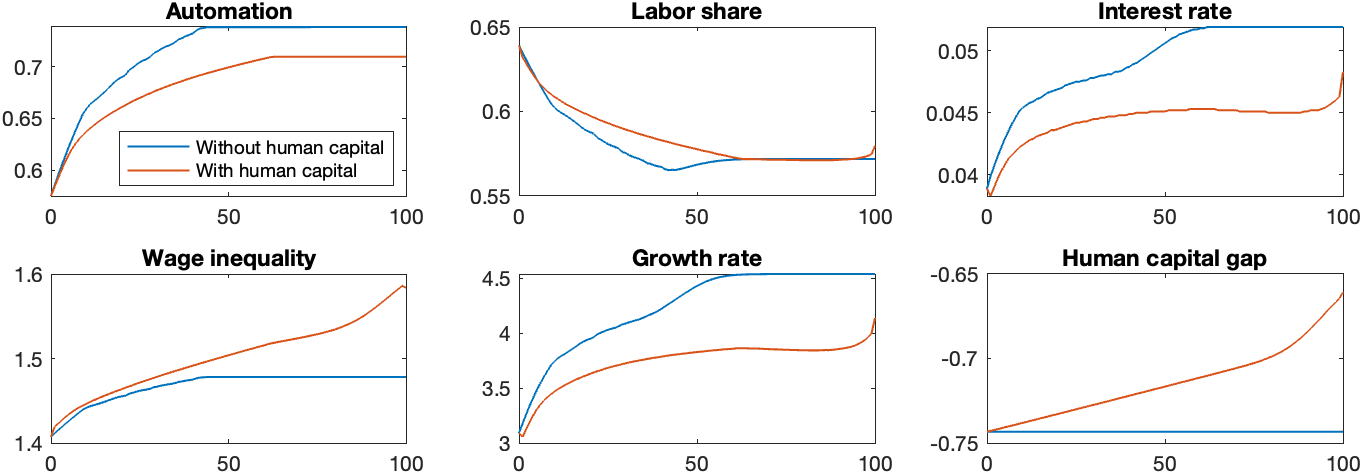
\includegraphics[width=\textwidth]{Transition}
\caption{Transition Path}
\label{transition}
{\scriptsize Notes: Simulation of transition path after a reduction of automation cost with calibrated model. }
\end{figure}

Figure \ref{transition} plots the simulation result of the transition path with calibrated model. A reduction of automation cost increases immediately the automation rate. 

However, the technology change increases the demand for capital but decrease the demand for both skilled and unskilled workers. As a result, the capital rental rate increases and wages decreases. This price changes increase the innovation patent value and decrease the automation patent value. The innovation rate starts to raise and the automation rate slows down, and converges to a higher level than the initial growth rate. 

Once the innovation rate starts to catch up with the automation, workers 


\subsection{Optimal policy}
In section 4, I solve social planner's problem and discuss the externalities in decentralized economy. In the decentralized economy, R\&D sector automates too many tasks and skilled workers invest too much in the human capital. Two taxes are appropriate to correct the externalities and increase the overall social welfare: automation tax ($\tau_I$) and training tax on skilled workers ($\tau_{hH}$). Automation tax decreases the value of automation patent and lowers the automation level; training tax on skilled workers favors the unskilled workers and decreases the human capital accumulation of skilled workers. 

I address the quantitative implications with the calibrated model and consider a redistributive policy. I consider the case in which where all the workers receive equal transfers, which are financed by either automation tax or training tax on skilled workers in a revenue-neutral way. 


\section{Empirical Implications}
I study the implications of my model in the context of exposure to automation affecting the skill level and training time. I start by documenting the changes in skill level and human capital investment. Then I estimate the effect of automation on the human capital response, both at the industry and occupation levels. I finalize by exploring the heterogeneous responses of college graduates or higher (skilled workers) and high school graduates or lower (unskilled workers) to the technology change. 

At the industry level, I use the EU KLEMS (EU level analysis of capital, labor, energy, materials and service inputs) and use Total Factor Productivity (TFP) growth as an approximation of the automation process following Autor and Salomons (2018)\nocite{AutorSalomons2018}. After a reduction of automation costs, both automation and innovation rates will increase, leading to an increase in TFP. I use labor composition (share of college graduates) in the EU KLEMS to approximate human capital. 

At the occupation level, I use the automation occupational exposure constructed by Webb(2019)\nocite{Webb2019}, which measures how likely the workers in each occupation can be replaced by machine. I use the measure of skill level and importance in O*NET (Occupational Information Network) to approximate the human capital stock. I uses the training time in ATES (Adult Training and Education Survey) to measure the investment in human capital. 

\subsection{Changes in skill level and human capital investment}
In this subsection, I document the change in skill level and human capital investment. At the industry level, I focus on the change of labor composition (share of college graduates or higher); at the occupation level, I focus on the skill level change and the time spent on training. 
 
To explore the human capital change at the industry level, I use the EU KLEMS September 2017 release, an industry-level panel dataset covering all individual EU-28 countries and the United States from 1995 to 2015. The data set contains statistical data on the economic growth (value added, compensation to capital and labor, etc.) and labor market composition (compensation and employment share for high/median/low educated workers), and analytical data on the growth factors (TFP, capital services, hours worked, labor composition, etc.). 

Table \ref{Industry_trend} summarizes the change in the share of skilled workers (college graduates or higher) by industry. Between 1995 and 2015, the aggregate share of skilled workers increased. There are significant variations between industries; industries using more unskilled workers like agriculture and manufacturing experienced more labor composition change, while industries using more skilled workers like education and health experienced less. First, workers respond to the change of technology by investing more in the human capital. Second, as shown in Restrepo (2015)\nocite{Restrepo2015}, automation replaces unskilled workers, and unskilled workers relocate to the industries that are less exposed to automation. In the subsection 6.2, I will estimate the effect of automation on labor composition, whiling controlling the relocation effect. 

\begin{table}[h!]
\begin{center}
\scriptsize
\begin{tabular}{l|cccc} 
\hline \hline
& \multicolumn{4}{c}{$100 \times$Annualized log change} \\
Industry & 1995 & 2000 & 2005 & 2010  \\ \hline
Accommodation and food service activities & -4.621 & 5.880 & 3.514 & 6.990 \\
Agriculture, forestry and fishing & 7.564 & 8.061 & 5.722 & 2.950 \\ 
Arts, entertainment and recreation & 5.433 & 4.225 & 3.221 & 2.307 \\
Construction & 2.375 & 2.481 & 2.821 & 3.721 \\
Education & 0.836 & 0.263 & 1.071 & 1.127 \\
Electricity, gas, steam and air conditioning supply & -0.389 & 1.290 & 3.568 & 3.925 \\
Financial and insurance activities & 2.248 & 1.412 & 1.669 & 3.753 \\
Health and social work & 2.564 & 0.822 & 1.937 & 2.432 \\
Information and communication & 3.194 & 1.934 & 3.660 & 2.844 \\
Mining and quarrying & 6.689 & 3.550 & 4.495 & 6.311 \\
Other service activities & 3.793 & 4.261 & 3.511 & 3.300 \\
Professional, scientific, technical, administrative & \multirow{2}{*}{1.491} & \multirow{2}{*}{1.358} & \multirow{2}{*}{1.335} & \multirow{2}{*}{2.495} \\
and support service activities &&&&\\
Public administration and defense,  & \multirow{2}{*}{2.186} & \multirow{2}{*}{2.553} & \multirow{2}{*}{2.808} & \multirow{2}{*}{2.806}\\
compulsory social security &&&&\\
Real estate activities & 3.613 & 2.000 & 3.091 & 2.656 \\
Total manufacturing & 3.884 & 2.619 & 4.248 & 3.707 \\
Transportation and storage & 2.991 & 2.305 & 6.175 & 4.027 \\
Water supply, sewerage,  & \multirow{2}{*}{3.532} & \multirow{2}{*}{2.446} & \multirow{2}{*}{1.437} & \multirow{2}{*}{4.999}  \\
waste management and remediation activities &&&&\\
Wholesale and retail trade & \multirow{2}{*}{3.984} & \multirow{2}{*}{2.603} & \multirow{2}{*}{2.770} & \multirow{2}{*}{4.607} \\
repair of motor vehicles and motorcycles &&&&\\
Total & 2.854  & 2.781 & 3.172  & 3.609 \\\hline
\end{tabular}
\end{center}
\caption{Trends in Skilled Worker Share by Industry}
\label{Industry_trend}
{\scriptsize Notes: Data are from the EU KLEMS (EU level analysis of capital, labor, energy, materials and service inputs). I calculate the average change of skilled worker share for the following periods: 1995-1999, 2000-2004, 2005-2009, 2010-2014.}
\end{table}

To explore the skill change at the occupation level, I use the O*NET (Occupational Information Network) data. I merge all the history releases of O*NET and construct panel data. For each occupation, O*NET measures the importance and level of different skills and updates the data almost twice a year. The first official O*NET data set was released in 2003, and a major change was made in 2010. In other releases, only a subset of occupations was updated. There are two groups of skills: basic skills, including content and process; cross-functional skills, including complex problem solving, resource management, social, systems and technical. Each subgroup includes several detailed skill types, which describe the specifically developed capacities needed for the occupation. 

Figure \ref{trend} summarizes the changes in importance and level for each skill group. Between 2000 and 2020, the trends in level and importance are very similar. The main change happened between 2002 and 2010, and only minor changes were made after the major update in 2010. The level and importance of social skill have grown significantly faster than other skills, while the technical skill is the only skill that is lower and less important than before. 

\begin{figure}[h!]
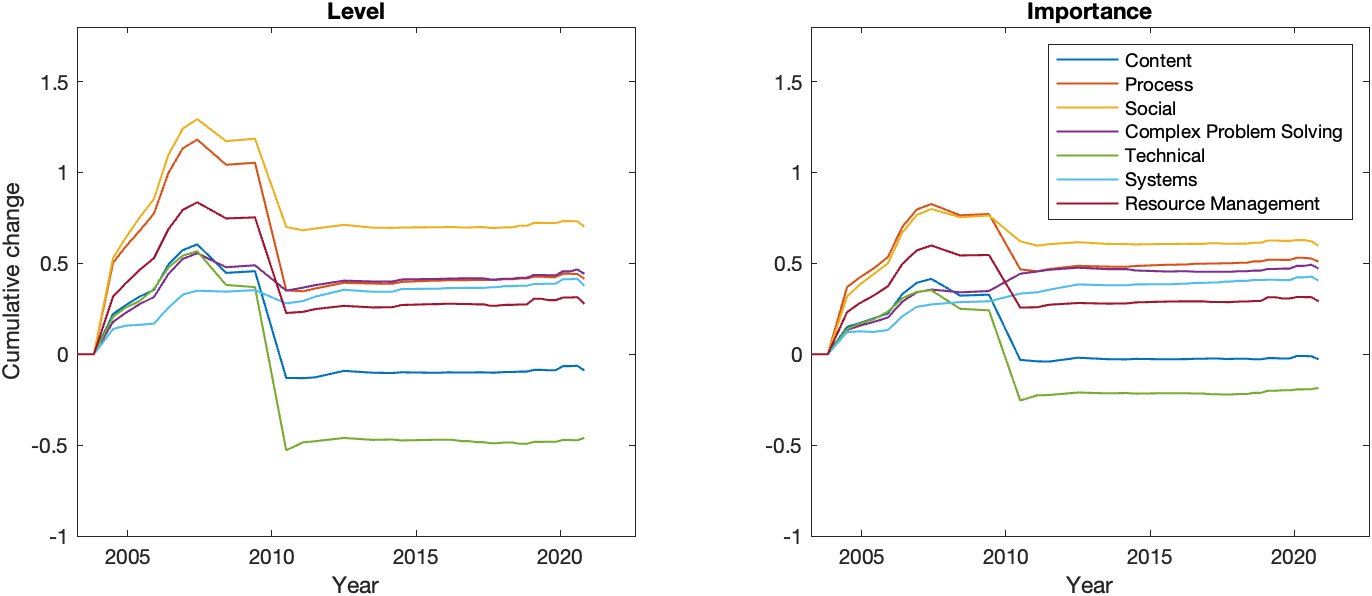
\includegraphics[width = \textwidth]{trend}
\caption{Trends in Skill Level and Importance}
\label{trend}
{\scriptsize Notes: Data are from the O*NET (Occupational Information Network). I calculate the average skill level or importance for the 7 skill groups. The xaxis is the release date of the data, the yaxis is the change of skill level or importance compared with the first release. }
\end{figure}

To see if automation exposure affects the human capital accumulation as predicted in the model, I partition the occupations into groups with low (under 33 percentile), median (between 33 and 66 percentile) and high (above 66 percentile) automation exposures. To do so, I use the automation occupational exposure measure constructed by Webb(2019)\nocite{Webb2019}. He uses the overlap between the text of job task descriptions (O*NET) and the text of patents (Google Patents Public Data) to measure the exposure of tasks to automation. The measure ranges from 0 to 100, indicating how likely the labor may be displaced at each occupation. Figure \ref{LV_trend1} summarizes the change in level for each skill group facing different automation exposure. The skill levels of all the skill groups increase significantly more when the occupation is more exposed to the automation. 

\begin{figure}[h!]
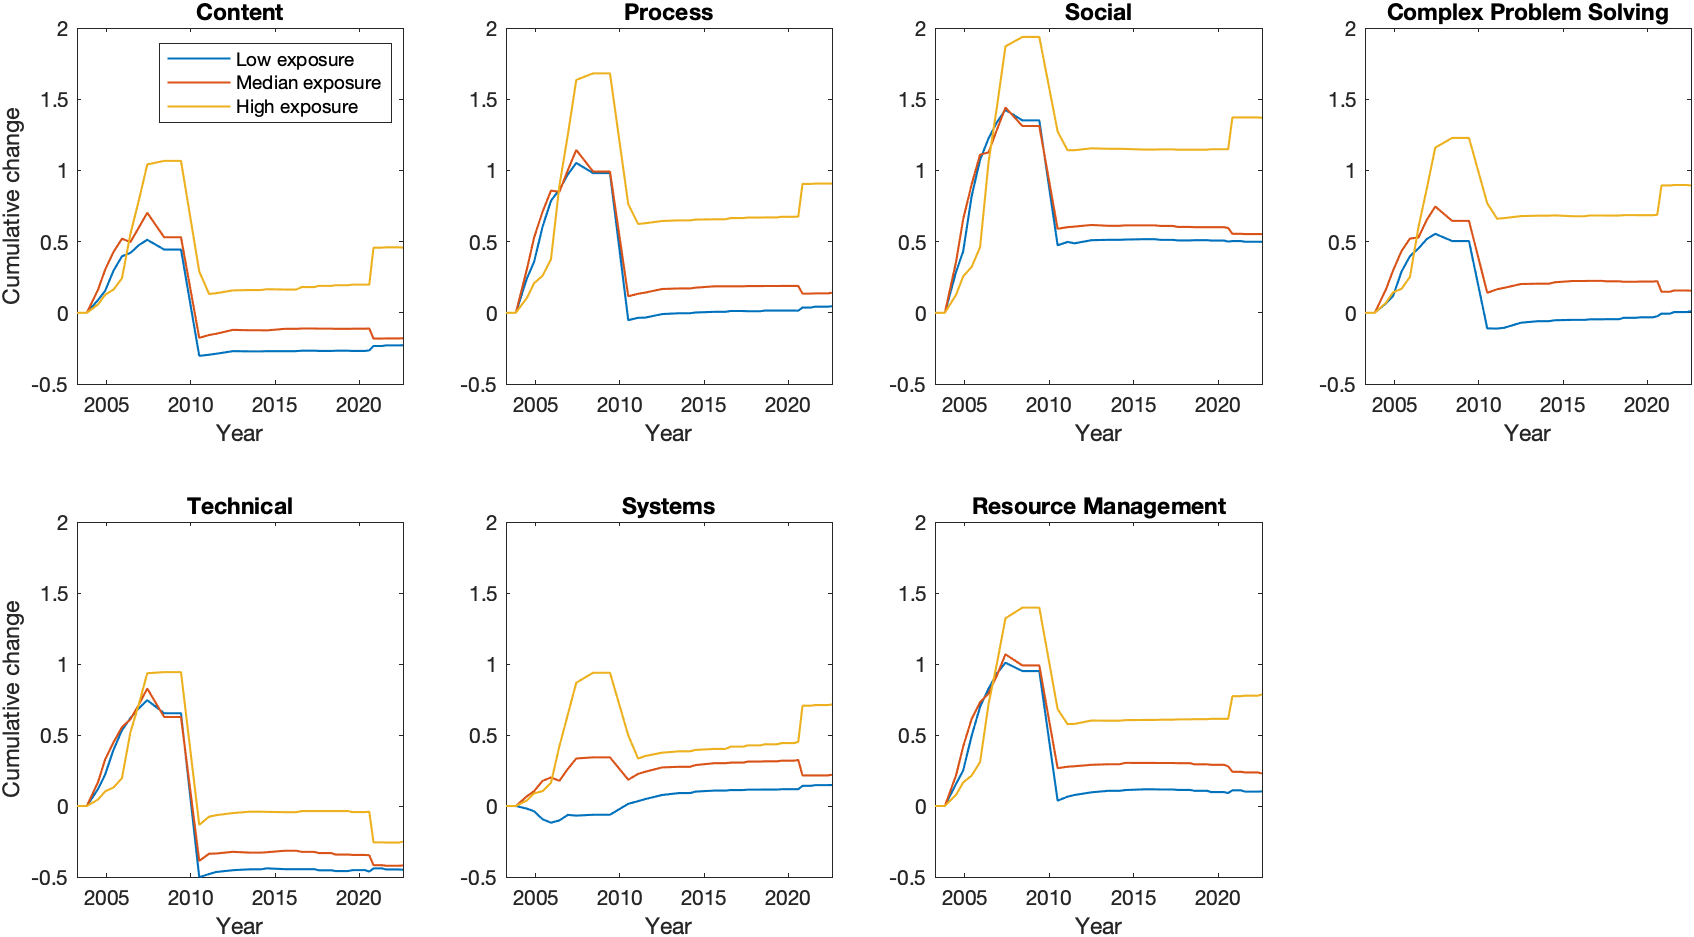
\includegraphics[width = \textwidth]{LV_trend1}
\caption{Trends in Skill Level Facing Different Automation Exposure}
\label{LV_trend1}
{\scriptsize Notes: Data are from the O*NET (Occupational Information Network). I partition the occupations into groups with low (under 33 percentile), median (between 33 and 66 percentile) and high (above 66 percentile) automation exposures, then I calculate the average skill level or importance for the 7 skill groups. The xaxis is the release date of the data, the yaxis is the change of skill level compared with the first release. }
\end{figure}

Another important empirical implication of my model is the heterogeneous responses of different skill groups. I partition the occupations into groups with low (under 33 percentile), median (between 33 and 66 percentile) and high (above 66 percentile) education levels. The education level is measured by the share of skilled workers working in the occupation. O*NET provides detailed information on workers' education level for each occupation, I construct the ratio of workers with a college degree or higher as the empirical analog of the share of skilled workers. Figure \ref{LV_trend2} summarizes the change in level for each skill group with different education levels. The skill levels of occupation grows faster as more skilled workers working at this occupation. 

\begin{figure}[h!]
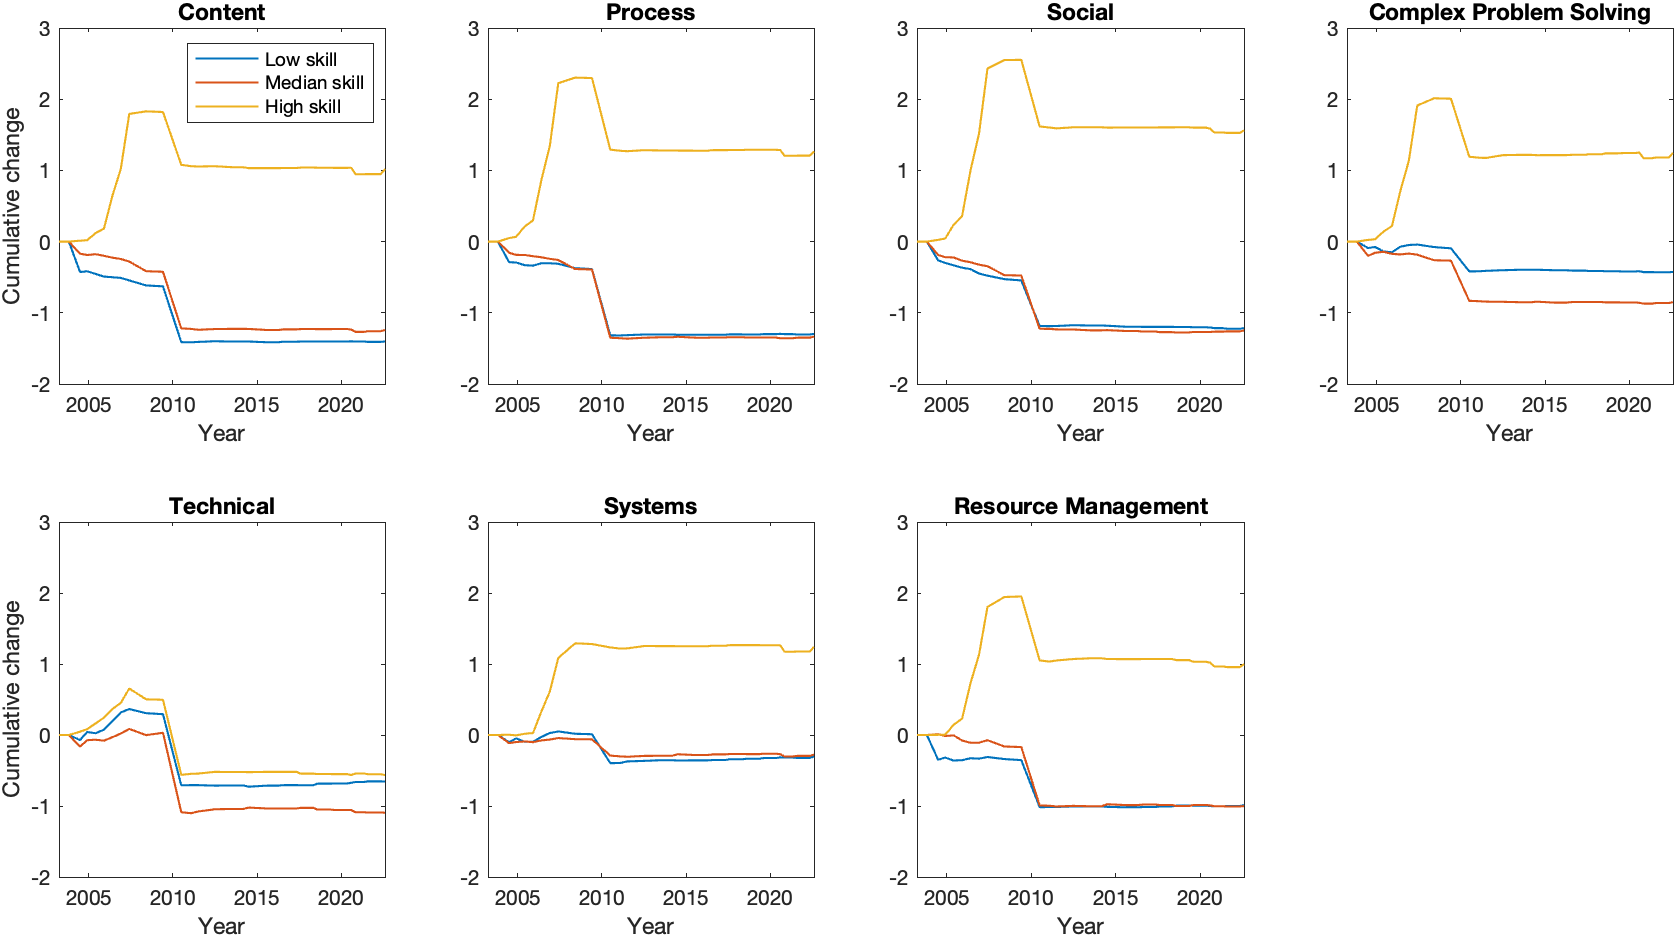
\includegraphics[width = \textwidth]{LV_trend2}
\caption{Trends in Skill Level with Different Education level}
\label{LV_trend2}
{\scriptsize Notes: Data are from the O*NET (Occupational Information Network). I partition the occupations into groups with low (under 33 percentile), median (between 33 and 66 percentile) and high (above 66 percentile) education, then I calculate the average skill level or importance for the 7 skill groups. The xaxis is the release date of the data, the yaxis is the change of skill level compared with the first release. }
\end{figure}

Direct measure of human capital investment can be constructed using ATES (Adult Training and Education Survey). The ATES collects data about adults ages 16 to 65 who are not enrolled in high school. I use the hours per week in ESL (English as a Second Language) and ABE (Adult Basic Education)/GED (General Equivalency Diploma) classes multiplied by number of weeks spent to construct the total hours spent on nondegree credentials. ATES also asks about the total hours spent on work experience programs. Other relevant data provided by ATES are: hours per week worked for pay, worker's occupation (20 aggregate groups) if employed, sex and age. 

Figure \ref{trend} plots the average training-working time ratio and the ratio of workers participating in any types of training for each occupation. Both ratios are decreasing in the automation exposure 
\begin{figure}[h!]
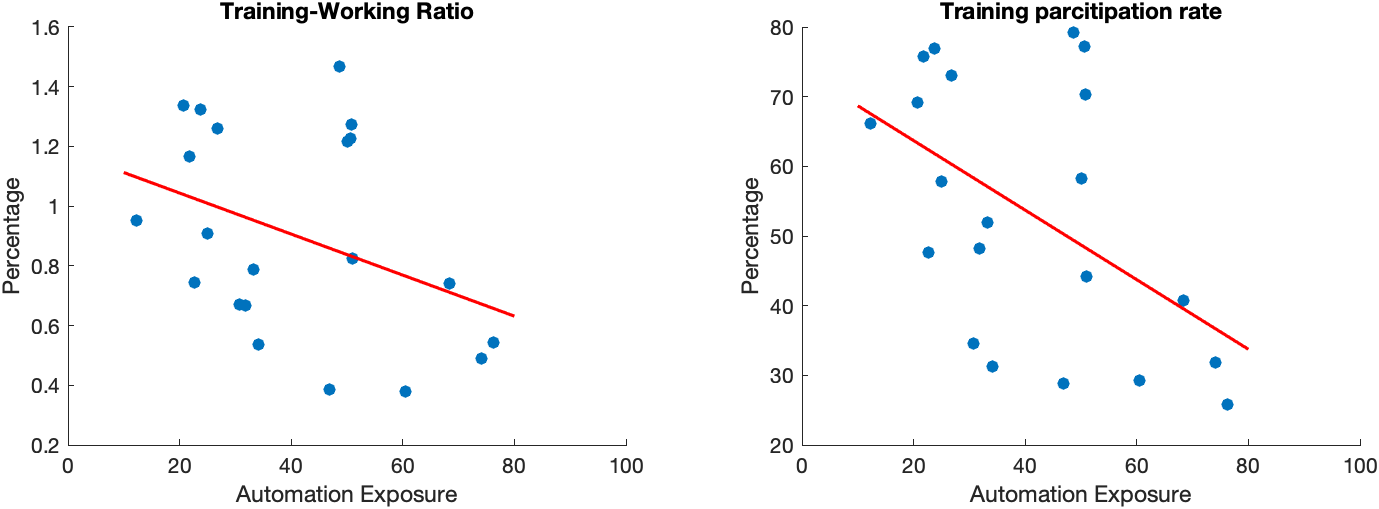
\includegraphics[width = \textwidth]{train}
\caption{Training Facing Different Automation Exposure}
{\scriptsize Notes: Data are from the ATES (Adult Training and Education Survey). I calculate the average training-working time ratio and the ratio of workers participating in any types of training for each occupation. The xaxis is the automation occupational exposure constructed by Webb (2019).}
\label{train}
\end{figure}

In this subsection, I document the change of labor composition and skill level over time. When a industry or occupation is exposed to automation, it experiences a faster change in labor composition or skill level. The faster change can be a result of higher human capital investment, or relocation between industries and allocations. Time spent on training can be a direct measure of human capital investment. Workers spend less time on training when their occupations are more exposed to automation. 

\subsection{Effects of Automation on Human Capital Investment}
Based on the prediction of the model, after a reduction of automation cost, both automation and innovation rates increase. In the long run, workers respond to the change in technology by investing more in their human capital. As a result, we should observe an increase in human capital or an improvement in labor composition (higher ratio of skilled workers). To test the correlation between automation and human capital growth, I use EU KLEMS data and estimate the equation:
\begin{align}
\begin{split}
 \Delta \ln Y_{i c, t-1} &=\beta_{0}+\beta_{1} \Delta \ln TFP_{i, c \neq c(i), t-k} +\beta_{2} \Delta \ln TFP_{i, c \neq c(i), t-k-1}+\beta_{3} \Delta \ln Y_{i c, t-2}\\
 &+\Delta L_{i c, t-1}+\alpha_{c}+\gamma_{t}+\epsilon_{ict}.
 \end{split}
\end{align}
I regress the outcome variable $\Delta \ln Y_{i c, t-1}$ on the TFP growth rate $\Delta \ln TFP_{i, c \neq c(i), t-k}$ with time leg $k \in \{1,2,3,4,5\}$ while controlling the lagged values of both TFP growth $\Delta \ln TFP_{i, c \neq c(i), t-k-1}$ and of outcome variable growth $\Delta \ln Y_{ic, t-2}$. In order to interpret $\beta_{1}$ as the effect of automation on human capital, not a result relocation, I control for the change of employment $\Delta L_{i c, t-1}$. I also control for the fixed effect of country $\alpha_{c}$ and year $\gamma_{t}$. In order to overcome the endogeneity between TFP and labor composition, I follow Autor and Salomons (2018)\nocite{AutorSalomons2018}, and construct industry-level TFP growth for each industry-country pair as the leave-out mean of industry-level TFP growth in all other countries, then rescaled it to have a unit standard deviation. The coefficient $\beta_{1}$ measures the impact of TFP growth on outcome variable with different lags. 

To measure human capital growth, I use two related variables: the change in the share of skilled workers (college graduates) and the growth rate contributed by labor composition change. The estimation result is reported in Table \ref{estimation1} and \ref{estimation2}. The coefficient $\beta_{1}$ is not significant except when $k=4$. The TFP growth does not immediately impact the labor composition but has a positively effect with a four-year lag. A one standard deviation positive TFP shock increases the share of skilled workers by 0.55\% and increases the growth rate contributed by labor composition change by 0.28\% after four years. 

\begin{table}[h!]
\begin{center}
\scriptsize
\begin{tabular}{lcccccc} \hline \hline
 & (1) & (2) & (3) & (4) & (5) & (6)\\
VARIABLES & \multicolumn{6}{c}{$100 \times$Annualized log change in share of skilled workers} \\ \hline
 &  &  &  &  &  &  \\
TFP Growth & -0.219 &  &  &  &  &  \\
 & (0.311) &  &  &  &  &  \\
TFP Growth (lag 1) &  & 0.339 &  &  &  &  \\
 &  & (0.252) &  &  &  &  \\
TFP Growth (lag 2) &  &  & 0.310 &  &  &  \\
 &  &  & (0.251) &  &  &  \\
TFP Growth (lag 3) &  &  &  & -0.253 &  &  \\
 &  &  &  & (0.257) &  &  \\
TFP Growth (lag 4) &  &  &  &  & 0.550** &  \\
 &  &  &  &  & (0.271) &  \\
TFP Growth (lag 5) &  &  &  &  &  & -0.412 \\
 &  &  &  &  &  & (0.282) \\
Constant & 4.305 & 4.655** & 5.924*** & 7.012*** & 7.012*** & 9.188*** \\
 & (2.770) & (1.971) & (1.963) & (1.987) & (2.033) & (2.090) \\
 &  &  &  &  &  &  \\
Observations & 2,301 & 2,657 & 2,325 & 1,993 & 1,661 & 1,330 \\
 R-squared & 0.120 & 0.123 & 0.135 & 0.151 & 0.178 & 0.223 \\ \hline
\end{tabular}
\end{center}
\caption{TFP Effect on High Educated Labor Share}
\label{estimation1}
{\scriptsize Date are from EU KLEMS. The table presents estimates of the incidence of TFP growth on labor composition change. Coefficients are for observed TFP shocks in $t = \{0,-1,-2,-3,-4,-5\}$, rescaled to have a unit standard deviation. Robust standard errors are in parenthesis. ***, **, * denotes statistical significance at 1, 5 and 10 percent levels.}
\end{table}

\begin{table}
\begin{center}
\scriptsize
\begin{tabular}{lcccccc} \hline \hline
 & (1) & (2) & (3) & (4) & (5) & (6)\\
VARIABLES & \multicolumn{6}{c}{Labor composition growth} \\ \hline
 &  &  &  &  &  &  \\
TFP Growth & -0.0787 &  &  &  &  &  \\
 & (0.0739) &  &  &  &  &  \\
TFP Growth (lag 1) &  & 0.0997 &  &  &  &  \\
 &  & (0.0806) &  &  &  &  \\
TFP Growth (lag 2) &  &  & 0.171** &  &  &  \\
 &  &  & (0.0864) &  &  &  \\
TFP Growth (lag 3) &  &  &  & 0.107 &  &  \\
 &  &  &  & (0.0941) &  &  \\
TFP Growth (lag 4) &  &  &  &  & 0.281** &  \\
 &  &  &  &  & (0.109) &  \\
TFP Growth (lag 5) &  &  &  &  &  & 0.0879 \\
 &  &  &  &  &  & (0.121) \\
Constant & -0.817 & -0.924 & -1.093 & -1.301 & -1.389 & -1.610 \\
 & (0.726) & (0.752) & (0.800) & (0.850) & (0.933) & (0.997) \\
 &  &  &  &  &  &  \\
Observations & 2,597 & 2,300 & 2,003 & 1,706 & 1,409 & 1,113 \\
 R-squared & 0.193 & 0.189 & 0.195 & 0.218 & 0.221 & 0.280 \\ \hline
\end{tabular}
\end{center}
\caption{TFP Effect on Labor Composition Growth}
\label{estimation2}
{\scriptsize Data are from the EU KLEMS. The table presents estimates of the incidence of TFP growth on growth rate contributed by labor composition change. Coefficients are for observed TFP shocks in $t = \{0,-1,-2,-3,-4,-5\}$, rescaled to have a unit standard deviation. Robust standard errors are in parenthesis. ***, **, * denotes statistical significance at 1, 5 and 10 percent levels.}
\end{table}

To estimate the effect of automation on labor composition more structurally, I adopt simple local projection models in Autor and Salomons (2018)\nocite{AutorSalomons2018}. They documented well in their paper the impact of automation on employment, hours worked, wage bills, and labor share. I adopt their estimation method while the outcome of interest is the labor composition and the growth rate contributed by labor composition change. I estimate the equation: 
\begin{align}
\begin{split}
\ln Y_{i c, t+K}-\ln Y_{i c, t-1}&=\beta_{0}+\beta_{1} \Delta \ln TFP_{i, c \neq c(i), t-1}+\sum_{k=0}^{K} \beta_{2}^{k} \Delta \ln TFP_{i, c \neq c(i), k} \\
&+\beta_{3} \Delta \ln T F P_{i, c \neq c(i), t-2}+\beta_{4} \Delta \ln Y_{i c, t-2}+\alpha_{c}+\gamma_{t}+\epsilon_{ict}
\end{split}
\end{align}
where $\ln Y_{i c, t+K}-\ln Y_{i c, t-1}$ represents the log change in share of high educated labor in industry $i$ and country $c$, from year $t-1$ to year $t+K$. The impulse variable is the log change in other-country-industry TFP between years $t-2$ and $t-1$, $\Delta \ln TFP_{i, c \neq c(i), t-1}$. I estimate the effects while controlling for lagged values of both TFP growth $\Delta \ln TFP_{i, c \neq c(i), t-2}$ and of outcome variable growth $\Delta \ln Y_{ic, t-2}$, and subsequent TFP innovations occurring between $t=0$ and $t=K$. I also control the fixed effect of country $\alpha_{c}$ and year $\gamma_{t}$. 

The estimation result is plotted in Figure \ref{LP}. Coefficients plotted in the figure are the response of outcomes to the TFP shock in $t = 0$. The trend is consistent with the result above, the TFP shock does not affect the labor composition immediately, but has long run effect on the human capital growth. The effect of TFP on human capital gradually increases overtime and peaks at five years after the shock. 

\begin{figure}[h!]
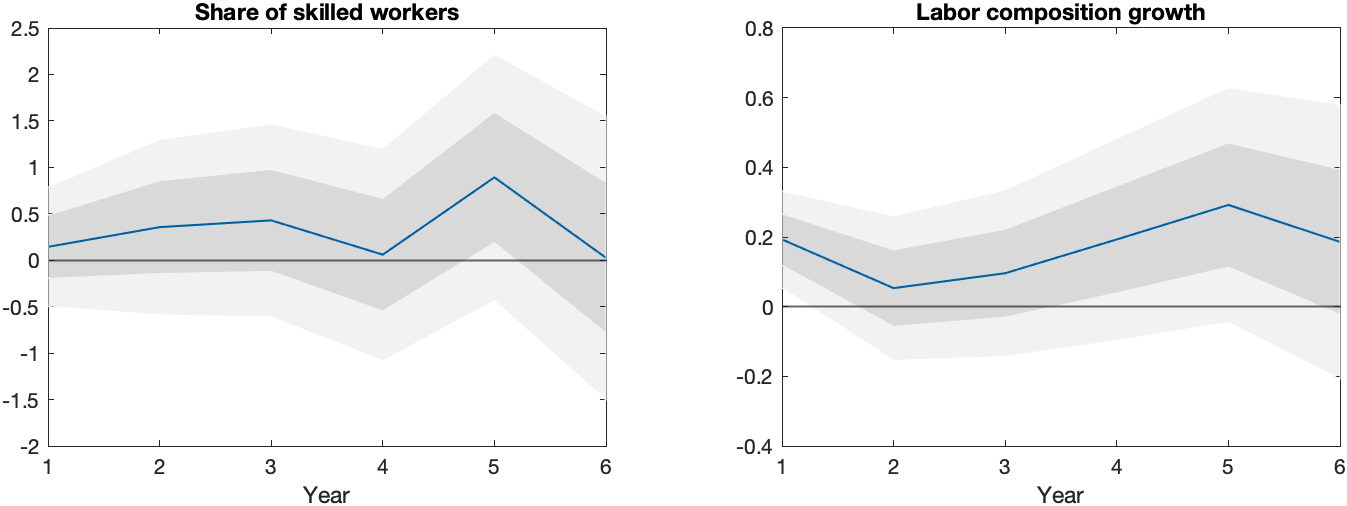
\includegraphics[width = \textwidth]{LP}
\caption{Local Projection Estimates of the Relationship Between TFP Growth and Human Capital}
\label{LP}
{\scriptsize Notes: Data are from the EU KLEMS. The figure presents estimates of the incidence of TFP growth on labor composition or growth rate contributed by labor composition change. Coefficients are for responses of the outcome variables at $t = \{1,2,3,4,5,6\}$ to observed TFP shocks in $t = 0$. TFP shocks are rescaled to have a unit standard deviation. Bands are 95\% and 70\% CI.}
\end{figure}

\subsection{Heterogeneous response}
The key empirical implication of my model is that, the skilled and unskilled workers respond differently to automation. First, automation benefit skilled workers more than unskilled workers. Second, skilled workers have better ability of learning. Using O*NET data, I estimate the equation: 
\begin{align}
\begin{split}
\log(y_{ijt}) &= \beta_0 t +\beta_1 t \times AOE_{i} + \beta_2 t \times EDUC_{it} +\beta_3 t \times AOE_{i} \times EDUC_{it} \\
&+ \alpha t \times 1\{t\ge 2001\} +\Gamma_j + \epsilon_{ijt}
\end{split}
\end{align}
$y_{ijt}$ represents the level of a skill $j$ for occupation $i$ at time $t$. $AOE$ is the automation occupational exposure for occupation $i$. $EDUC$ is the ratio of skilled workers (college graduate or higher) at occupation $i$. $t$ is the time trend, $t\times AOE_{i}$, $t\times EDUC_{it}$ and $t\times AOE_{i}\times EDUC_{it}$ are interaction between time trend and automation or education level. The effect is estimated while controlling the time trend and fixed effect for each skill $j$. I also use the term $t \times 1\{t\ge 2001\}$ to control the major change happened in 2001. 

$\beta_1$ and $\beta_2$ are interpreted as the effects of automation and education on skill level growth. The key coefficient of the regression is $\beta_3$, it captures the different human capital responses of skilled and unskilled workers facing automation. The estimation result is reported in Table \ref{estimation3}. The level for all the skills except technical skill are increasing overtime. Consistent with the predictions of my model, when the workers are more exposed to automation, they have less incentive to invest in their human capital due to the displacement effect. Skilled and unskilled workers respond differently to the exposure of automation, skilled workers increase their human capital investment more than the unskilled workers. 

The result is consistent with the empirical result of Acemoglu et al.(2020)\nocite{Acemogluetal2020}. Robots adopters experience a decline on the share of production workers, but increase the overall employment. When an occupation is exposed to automation, the skill levels of the occupation change differently depending on the labor composition. If the workers at this occupation is mainly unskilled workers, they get displaced and their human capital accumulation gets slow down. If the workers at the occupation is mainly skilled workers, they experience a productivity gain, and increase their human capital accumulation to adapt to the technology change. 
\begin{table}[h!]
\begin{center}
\scriptsize
\begin{tabular}{lccccccc} \hline \hline
 & (1) & (2) & (3) & (4) & (5) & (6) & (7) \\
Skill group & Content & Process & Social & Problem& Technical & Systems & Resource\\ 
 & &  & & Solving &  & & Management \\ \hline
 &  &  &  &  &  &  &  \\
t & 0.287*** & 0.345*** & 0.276*** & 0.0852*** & 0.152*** & -0.0570*** & 0.408*** \\
 & (0.00971) & (0.00578) & (0.00498) & (0.00934) & (0.0143) & (0.00979) & (0.0133) \\
t $\times$ AOE& -0.109*** & -0.0811*** & -0.165*** & -0.0392*** & 0.538*** & -0.103*** & -0.116*** \\
 & (0.00316) & (0.00189) & (0.00158) & (0.00321) & (0.00485) & (0.00326) & (0.00443) \\
t $\times$ EDUC & 0.211*** & 0.185*** & 0.103*** & 0.187*** & 0.0949*** & 0.231*** & 0.145*** \\
 & (0.00294) & (0.00178) & (0.00149) & (0.00301) & (0.00470) & (0.00306) & (0.00414) \\
t $\times$ AOE $\times$ EDUC & 0.278*** & 0.0543*** & 0.104*** & 0.0841*** & 0.240*** & 0.188*** & 0.341*** \\
 & (0.00627) & (0.00383) & (0.00321) & (0.00649) & (0.00967) & (0.00659) & (0.00883) \\
Constant & 130.4*** & 127.4*** & 118.7*** & 116.1*** & 68.18*** & 124.4*** & 115.0*** \\
 & (0.714) & (0.371) & (0.368) & (0.396) & (1.251) & (0.570) & (0.850) \\
 &  &  &  &  &  &  &  \\
Observations & 216,494 & 147,206 & 220,769 & 36,802 & 324,869 & 110,293 & 144,779 \\
 R-squared & 0.521 & 0.478 & 0.413 & 0.432 & 0.237 & 0.406 & 0.471 \\ \hline
\end{tabular}
\end{center}
\caption{Effect of Automation on Skill Level}
\label{estimation3}
{\scriptsize Notes: Data are from the O*NET (Occupational Information Network). The table presents estimates of the incidence of automation and education on the skill level of different skill groups. $t$ is the time trend, $t\times AOE_{i}$, $t\times EDUC_{i}$ and $t\times AOE_{i}\times EDUC_{i}$ are interaction between time trend and automation or education level.I control for the time trend and fixed effect for each skill. Robust standard errors are in parenthesis. ***, **, * denotes statistical significance at 1, 5 and 10 percent levels.}
\end{table}

Similar pattern can be found using the direct measure of human capital investment. Using ATES data, I estimate the equation: 
\begin{align}
\log (y) = \beta_0 t +\beta_1 t \times AOE + \beta_2 t \times SKILL +\beta_3 t \times AOE \times SKILL + \Gamma + \epsilon
\end{align}
$y$ represents total hour spent on training. $AOE$ is the automation occupational exposure for the worker's occupation. $SKILL$ is the skill group of the worker (1 if the skilled and 0 if unskilled). $t$ captures the time trend of the time spent on training, $t\times AOE$, $t\times EDUC$ and $t\times AOE\times EDUC$ are interaction between time trend and automation or skill level. $\Gamma$ is the vector of control variables, including age and sex. 

The key coefficient of the regression is $\beta_3$, it captures the different training responses of skilled and unskilled workers facing automation. The estimation result is reported in Table \ref{estimation4}. The result is consistent with the occupational skill level change above, workers working at occupations that are more exposed to automation invest less in training, skilled workers invest more in training than unskilled workers. With 1 percent increase of automation level, skilled workers increase their training time about 0.035\% more than unskilled workers. 

\begin{table}[h!]
\begin{center}
\scriptsize
\begin{tabular}{lcc} \hline \hline
 & (1) & (2) \\
VARIABLES & \multicolumn{2}{c}{Training hours} \\ \hline
 &  &  \\
t  & 1.754*** & 1.843*** \\
 & (0.00183) & (0.00183) \\
t $\times$ AOE & -0.0145*** & -0.0240*** \\
 & (5.61e-05) & (5.65e-05) \\
t $\times$ SKILL & 0.00752*** & 0.00575*** \\
 & (2.90e-05) & (2.89e-05) \\
t $\times$ AOE $\times$ SKILL & 0.0341*** & 0.0352*** \\
 & (7.96e-05) & (7.93e-05) \\
Constant & -3,210*** & -3,336*** \\
 & (3.661) & (3.649) \\
 &  &  \\
Observations & 129,673,600 & 129,673,600 \\
 R-squared & 0.032 & 0.042 \\ \hline
\end{tabular}
\end{center}
\caption{Effect of Automation on Training}
\label{estimation4}
{\scriptsize Notes: Data are from the ATES (Adult Training and Education Survey). The table presents estimates of the incidence of automation and education on training hours (Weighted least squares). $t$ is the time trend, $t\times AOE$, $t\times SKILL$ and $t\times AOE\times SKILL$ are interaction between time trend and automation or skill level. In the second column, I control for the sex and age. Robust standard errors are in parenthesis. ***, **, * denotes statistical significance at 1, 5 and 10 percent levels.}
\end{table}

\section{Conclusion}

This paper discusses the responses of human capital to a reduction of automation cost. When the technological revolution lowers the cost of automation, it immediately increases automation, displaces workers and lowers the wage growth rage. The higher automation level improves the production factor allocation and increases the innovation incentives of the R\&D sector. The innovation rate catches up with the automation rate and encourages human capital investment. Higher human capital growth rate increases the effective labor supply, substituting automation and complementing innovation. With endogenous human capital responses, the economy converges to a balanced growth path with lower automation level and higher labor share compared with the scenario without human capital channel. However, skilled workers respond more than unskilled workers to the technological revolution. Skilled workers benefit more from the productivity effect while unskilled workers affected more by the displacement effect. Skilled workers also have more ability to adjust their human capital investment. The uneven responses amplify the wage inequality.

My data supports the implications of this mechanism. High exposure to automation decreases the human capital investment incentives. Skilled workers adjust more than unskilled workers in the human capital facing the automation exposure. 

Theories and data suggest that the new technological changes are skill-biased and complements skilled workers (Violante, 2018\nocite{Violante2008}). In my model, I assume constant elasticity of substitution between production factors, which could underestimate the uneven effect of automation on different skill groups. The allocation friction of unskilled workers can also contribute to the inequality after an increase of automation level. Another extension of my model is to consider multi-dimensional skills; as shown in the empirical section, each skill group responds differently to the ongoing technological changes. 

\clearpage
\bibliographystyle{plain}
\bibliography{Growth}
\clearpage

\begin{appendices}

\section{Firm Problem}

\subsubsection*{Final Good Producer}
The competitive final good producers solve the following problem 
\begin{align*}
\max \quad & Y-\int_{N-1}^Np(i)y(i)di \\
&Y = \tilde{A}\Big(\int_{N-1}^{N}y(i)^{\frac{\sigma-1}{\sigma}}di\Big)^{\frac{\sigma}{\sigma-1}}
\end{align*}

Take first order condition with respect to $y(i)$
\begin{align*}
\tilde{A}\Big(\int_{N-1}^{N}y(i)^{\frac{\sigma-1}{\sigma}}di\Big)^{\frac{1}{\sigma-1}}y(i)^{-\frac{1}{\sigma}}-p(i) = 0
\end{align*}
Then the demand function of each task can be written as 
\begin{align*}
y(i) = \tilde{A}^{\sigma-1}Yp(i)^{-\sigma}
\end{align*}

\subsubsection*{Task Producer}
The task producers who have adopted machine solves the following problem 
\begin{align*}
\max \quad  p(i)&y(i)-Rk(i)-\psi q(i) \\
&y(i) = q(i)^{\eta}k(i)^{1-\eta}
\end{align*}
Take first order condition with respect to $k(i)$ and $q(i)$
\begin{align*}
q(i)\psi &= \eta p(i)y(i) \\
k(i)R &= (1-\eta)p(i)y(i) 
\end{align*}
The unit cost of production can be written as 
\begin{align*}
y(i) &= (\frac{\eta p(i)y(i)}{\psi})^{\eta}(\frac{(1-\eta)p(i)y(i)}{R})^{1-\eta} \\
p(i) &= (\frac{\psi}{\eta})^{\eta} (\frac{R}{1-\eta})^{1-\eta} \\
 	  &= \Psi R^{1-\eta}, \quad \Psi =  (\frac{\psi}{\eta})^{\eta} (\frac{1}{1-\eta})^{1-\eta}
\end{align*}
Plug in the demand function solved from final good producer problem, the output of the task $p(i)y(i)$ can then be solved 
\begin{align*}
p(i)y(i) = (\frac{\tilde{A}}{\Psi})^{\sigma-1}YR^{(1-\eta)(1-\sigma)} = Y(\frac{R}{A})^{1-\hat{\sigma}}
\end{align*}
Where $\hat{\sigma} = 1-(1-\eta)(1-\sigma)$ and $A = \Big(\frac{\tilde{A}}{\Psi}\Big)^{\frac{\sigma-1}{\hat{\sigma}-1}}  = \Big(\frac{\tilde{A}}{\Psi}\Big)^{\frac{1}{1-\eta}}$. 
The demand of capital for task $i$ is 
\begin{align*}
k(i) = (1-\eta)A^{\hat{\sigma}-1}YR^{-\hat{\sigma}}
\end{align*}
Similarly, the unit cost of task if the producers use unskilled or skilled workers can be solved as 
\begin{align*}
p(i) =
\begin{dcases}
\Psi(\frac{W_L}{\gamma_L(i,h_L)})^{1-\eta}, \quad \text{unskilled worker}  \\
\Psi(\frac{W_H}{\gamma_H(i,h_H)})^{1-\eta}, \quad \text{skilled worker}
\end{dcases}
\end{align*}
The output of the tasks $p(i)y(i)$ are
\begin{align*}
p(i)y(i) =
\begin{dcases}
Y(\frac{W_L}{A\gamma_L(i,h_L)})^{1-\hat{\sigma}}, \quad \text{unskilled worker}  \\
Y(\frac{W_H}{A\gamma_H(i,h_H)})^{1-\hat{\sigma}}, \quad \text{skilled worker}
\end{dcases}
\end{align*}
And the demand of unskilled and skilled workers can be solved as 
\begin{align*}
l(i) &= (1-\eta)A^{\hat{\sigma}-1}\frac{Y}{\gamma_L(i,h_L)}(\frac{W_L}{\gamma_L(i,h_L)})^{-\hat{\sigma}} \\
h(i) &= (1-\eta)A^{\hat{\sigma}-1}\frac{Y}{\gamma_H(i,h_H)}(\frac{W_H}{\gamma_H(i,h_H)})^{-\hat{\sigma}} 
\end{align*}
 
\section{Proposition Proofs}

\subsubsection*{Factor Allocation}
The research sector always automates the least updated tasks since they are the tasks where machine have less disadvantage. The research sector will develop the patent only if the firm can make more profit by adopting machine and is willing to purchase the patent. As a result, for all the task that are automated ($N-1 \le i \le I$), it must be true that 
\begin{align*}
R^{1-\eta} < \min \{(\frac{W_L}{\gamma_L(i,h_L)})^{1-\eta},(\frac{W_H}{\gamma_H(i,h_H)})^{1-\eta}\}
\end{align*}
And all the firms who have access to automation patent choose to produce the task using machine. 

For the tasks that are not automated, skilled workers always have advantage over more updated tasks. $\frac{W_H}{W_L}$ is increasing in $S$, when $S\to I$, $\frac{W_H}{W_L}\to 0$, when $S\to N$, $\frac{W_H}{W_L}\to \infty$. $ \frac{\gamma_H(S,h_L)}{\gamma_L(S,h_L)}$ is increasing in $S$. There exists a unique cutoff point $S$ such that 
\begin{align*}
\frac{W_H}{W_L} = \frac{\gamma_H(S,h_L)}{\gamma_L(S,h_L)}
\end{align*}
Then, for other tasks that are not automated, we get 
\begin{align*}
\frac{W_H}{\gamma_H(i,h_L)}\frac{\gamma_L(i,h_L)}{W_L} = e^{(B-B_N)(S-i)}\frac{W_H}{\gamma_H(S,h_L)}\frac{\gamma_L(S,h_L)}{W_L} =  e^{(B-B_N)(S-i)}
\end{align*}

If $i<S$, then $\frac{W_H}{\gamma_H(i,h_L)}\frac{\gamma_L(i,h_L)}{W_L}>1$, the firm will choose to produce the task using unskilled workers. If $i>S$ then $\frac{W_H}{\gamma_H(i,h_L)}\frac{\gamma_L(i,h_L)}{W_L}<1$, the firm will choose to produce the task using skilled workers.

\subsubsection*{Aggregate Production Function}
At equilibrium, the market clearing condition needs to be satisfied
\begin{align*}
K &= \int_{N-1}^I k(i)di=  \int_{N-1}^I(1-\eta)A^{\hat{\sigma}-1}YR^{-\hat{\sigma}}di \\
L_L &= \int_{I}^S l_L(i)di=  \int_{N-1}^I (1-\eta)A^{\hat{\sigma}-1}\frac{Y}{\gamma_L(i,h_L)}(\frac{W_L}{\gamma_L(i,h_L)})^{-\hat{\sigma}}di \\
L_H &=\int_{S}^N l_H(i)di=  \int_{N-1}^I (1-\eta)A^{\hat{\sigma}-1}\frac{Y}{\gamma_H(i,h_H)}(\frac{W_H}{\gamma_H(i,h_H)})^{-\hat{\sigma}} di
\end{align*}
Then the factor prices could be solved using market clearing condition 
\begin{align*}
R &=A\Gamma_K \Big(\frac{(1-\eta)Y}{A\Gamma_K K}\Big)^{\frac{1}{\hat{\sigma}}}, \quad \Gamma_K= (I-N+1)^{\frac{1}{\hat{\sigma}-1}}  \\
W_L &= A\Gamma_L\Big(\frac{(1-\eta)Y}{A\Gamma_LL_L}\Big)^{\frac{1}{\hat{\sigma}}}, \quad \Gamma_L=\Big(\frac{\gamma_L(S,h_L)^{\hat{\sigma}-1}-\gamma_L(I,h_L)^{\hat{\sigma}-1}}{B_L(\hat{\sigma}-1)}\Big)^{\frac{1}{\hat{\sigma}-1}}  \\
W_H &=A\Gamma_H\Big(\frac{(1-\eta)Y}{A\Gamma_HL_H}\Big)^{\frac{1}{\hat{\sigma}}}, \quad \Gamma_H = \Big(\frac{\gamma_H(N,h_H)^{\hat{\sigma}-1}-\gamma_H(S,h_H)^{\hat{\sigma}-1}}{B(\hat{\sigma}-1)}\Big)^{\frac{1}{\hat{\sigma}-1}} 
\end{align*}

Plug in the factor price and output for each task 
\begin{align*}
Y &= \int_{N-1}^N p(i)y(i) di \\
	&= \int_{N-1}^I Y(\frac{R}{A})^{1-\hat{\sigma}} di + \int_I^S Y(\frac{W_L}{A\gamma_L(i,h_L)})^{1-\hat{\sigma}} di  + \int_S^N Y(\frac{W_H}{A\gamma_H(i,h_H)})^{1-\hat{\sigma}} di \\
\Big(\frac{(1-\eta)Y}{A} \Big)^{\frac{\hat{\sigma}-1}{\hat{\sigma}}} &= \int_{N-1}^I \frac{(\Gamma_K K)^{\frac{\hat{\sigma}-1}{\hat{\sigma}}}}{\Gamma_K^{\hat{\sigma}-1}} di + \int_I^S \frac{(\Gamma_LL_L \gamma_L(i,h_L))^{\frac{\hat{\sigma}-1}{\hat{\sigma}}}}{\Gamma_L^{\hat{\sigma}-1}} di  + \int_S^N \frac{(\Gamma_HL_H \gamma_H(i,h_H))^{\frac{\hat{\sigma}-1}{\hat{\sigma}}}}{\Gamma_H^{\hat{\sigma}-1}} di 
 \end{align*}
The final good could be written as 
\begin{align*}
Y = \frac{A}{1-\eta}\Big((\Gamma_K K)^{\frac{\hat{\sigma}-1}{\hat{\sigma}}}+(\Gamma_LL_L)^{\frac{\hat{\sigma}-1}{\hat{\sigma}}}+(\Gamma_HL_H)^{\frac{\hat{\sigma}-1}{\hat{\sigma}}}\Big)^{\frac{\hat{\sigma}}{\hat{\sigma}-1}}
 \end{align*}

\subsubsection*{Human Capital Growth and Automation Level}
The long run interest rate needs to satisfy: 
\begin{align*}
r = \rho+\theta g = \rho+\theta(Bg_N+bg_{hH})
\end{align*}
Higher human capital growth rate increases the long run interest rate, which increases the innovation patent value and decreases the automation patent value. The automation level needs to decrease in order to have: 
\begin{align*}
\frac{p_N}{p_I} = (\frac{\mu_N}{\mu_I})^{\frac{1}{\lambda}}
\end{align*} 
 
\subsubsection*{Human Capital and Technology Growth Rate}
On the balanced growth path, the human capital investment needs to satisfy the following equation: 
\begin{align*}
(1-\theta)\frac{b}{\mu_hj}(1-l_j)^{\alpha_j}+\alpha\frac{b}{\mu_hj}l_j(1-l_j)^{\alpha_j-1} = \rho+(\theta-1)Bg_N
\end{align*}
Define $f(l)$ as the left hand side of the equation. 
\begin{align*}
f'(l) = \alpha_j\frac{b}{\mu_hj}(1-l_j)^{\alpha_j-1}\big(\theta+(1-\alpha_j)\frac{l_j}{1-l_j}\big)>0
\end{align*}
If $\theta-1>0$, the labor supply is increasing in $g_N$; If $\theta-1<0$, the labor supply is decreasing in $g_N$. 

\subsubsection*{Long-run comparative statistics}
On the balanced growth path, the value of patent needs to satisfy: 
\begin{align*}
\frac{p_N}{p_I} = (\frac{\mu_N}{\mu_I})^{\frac{1}{\lambda}}
\end{align*} 
The left hand side is increasing in the automation level. Higher automation level decrease the demand for labor and decreases the wage level. Lower wage level increases the innovation patent value $p_N$ and decreases the automation patent value $p_I$. The right hand side is decreasing in the cost of automation. When the automation cost decreases, the right hand side decreases, the automation level must increase. 

The number of scientist working on the innovation sector must satisfy: 
\begin{align*}
 \frac{\lambda\epsilon_N(t)^{\lambda-1}}{\mu_N}p_N(t) = \omega_H(t).
\end{align*} 
Higher automation level increases $p_N$ and increases the number of scientists working in the innovation sector. The innovation rate is higher. 

On the balanced growth path, the human capital of skilled and unskilled workers need to grow at the same rate $g_{hH} = g_{hL} = g_h$. Using the policy function for human capital investment, I can get:
\begin{align*}
\alpha_H((\mu_{hH}g_{hH})^{-\frac{1}{\alpha_H}}-1) = \alpha_L((\mu_{hL}g_{hL})^{-\frac{1}{\alpha_L}}-1)
\end{align*}

Then I can derive the ratio of human capital investment cost and human capital gap as:
\begin{align*}
\log(\frac{\mu_{hH}}{\mu_{hL}}) &= (\frac{\alpha_H}{\alpha_L}-1)\log(\mu_{hL}g_h)-\alpha_H\log((\frac{\alpha_H}{\alpha_L}-1)(\mu_{hL}g_h)^{\frac{1}{\alpha_L}}+1)-\log(\frac{\alpha_H}{\alpha_L}) \\
h_{HL}-h_{HL}^*&= -\frac{\alpha_H}{\lambda_h}\log \Big(\frac{\alpha_L(\mu_{hL}g_h)^{-\frac{1}{\alpha_L}}+\alpha_H-\alpha_L}{\alpha_H(\mu_{hL}g_h)^{-\frac{1}{\alpha_H}}}\Big)
\end{align*}
Take derivatives on $g_h$, I can get:
\begin{align*}
dh_{HL} = \frac{1}{\lambda_h}\frac{(\alpha_H-\alpha_L)l_L}{(1-l_L)\alpha_H+l_L\alpha_L}d\log g_h
\end{align*}

\section{Calibration}
To calibrate the parameters internally, I need to find the relevant moments. 
Discount rate $\rho$ can calibrated using the long-run interest rate and growth rate. 
\begin{align*}
r = \rho+\theta g
\end{align*}
Patent share $\eta$ is calibrated using the ratio of R\&D investment and GDP. 
\begin{align*}
\frac{W_H(\epsilon_N+\epsilon_I)}{Y} = (\frac{W_H}{Y})^{\frac{\lambda}{\lambda-1}}\Big((\frac{1}{\lambda}\frac{\mu_N}{p_N})^{\frac{1}{\lambda-1}}+(\frac{1}{\lambda}\frac{\mu_I}{p_I})^{\frac{1}{\lambda-1}}\Big) \propto \eta^{\frac{1}{1-\lambda}}
\end{align*}
Cost of innovation needs to set to match the innovation growth rate: 
\begin{align*}
g_N = (\frac{1}{\mu_N})^{\frac{1}{1-\lambda}}(\frac{\lambda P_N}{W_H})^{\frac{\lambda}{1-\lambda}} \propto (\frac{1}{\mu_N})^{\frac{1}{1-\lambda}}
\end{align*}
Capital productivity $A$ and cost of automation are calibrated using short run interest rate and capital share.  
\begin{align*}
R &= AH\Big(\frac{s_K}{1-\eta}\Big)^{\frac{1}{1-\hat{\sigma}}} \propto A \\
\frac{P_I}{P_N} &=(\frac{\mu_I}{\mu_N})^{\frac{1}{\lambda}} \propto \mu_I^{\frac{1}{\lambda}}
\end{align*}

Skill comparative advantage $B_H$ and training cost elasticity $\lambda_h$ is calibrated using wage premium in 1980 and 2005. 
\begin{align*}
\omega &= (\frac{\Gamma_H}{\Gamma_L})^{\frac{{\hat{\sigma}}-1}{\hat{\sigma}}} \\
d \ln \omega &=(B-B_L)d\tilde{S}+bdh_{HL}  \\
dh_{HL} &= \frac{1}{\lambda_h}\frac{(1-\frac{\alpha_L}{\alpha_H})l_L}{1-(1-\frac{\alpha_L}{\alpha_H})l_L}d\log(g_h) \propto \frac{1}{\lambda_h}
\end{align*}

Training law of motion $\alpha_H$ and $\alpha_L$ are calibrated using the change of training time. 
\begin{align*}
d\log(1-l_H) &= \frac{1}{(1-l_L)\alpha_H+l_L\alpha_L}d\log(g_h) \\
d\log(1-l_L) &= \frac{1}{\alpha_L}d\log(g_h) 
\end{align*}

Size of technology wave is calibrated to match the change of labor share. 
\begin{align*}
\frac{P_I}{P_N} =(\frac{\mu_I}{\mu_N})^{\frac{1}{\lambda}} \propto \mu_I^{\frac{1}{\lambda}}
\end{align*}

\section{Transition Path Algorithm}

To solve the transition path numerically between two balanced growth path. I firstly solve the BGP before and after political or technological shock, and use them as the starting and end point. 

\begin{itemize}
\item[(1)] Start with the initial guess of capital stock $\{k_0(t)\}$, labor supply $\{L_{H0}(t), L_{L0}(t)\}$, automation level $\{\tilde{I}_0(t)\}$, human capital gap $\{h_{HL0}(t)\}$ and growth rates $\{g_{N0}(t),g_{hH0}(t),g_{hL0}(t)\}$. 


\item[(2)] By solving firm's problem, I can get prices $\{r(t),\omega_H(t),\omega_L(t)\}$, capital and labor share $\{s_K(t),s_H(t),s_L(t)\}$
\begin{align*}
r &= A \Gamma_K(\frac{(1-\eta)y}{A\Gamma_Kk})^{\frac{1}{\hat{\sigma}}}-\delta \\
\omega_H &= A \tilde{\Gamma}_H(\frac{(1-\eta)y}{A\tilde{\Gamma}_HL_H})^{\frac{1}{\hat{\sigma}}} \\
\omega_L &= A \frac{\tilde{\Gamma}_L}{\gamma_{HL}}(\frac{(1-\eta)y}{A\frac{\tilde{\Gamma}_L}{\gamma_{HL}}L_L})^{\frac{1}{\hat{\sigma}}} \\
s_K &= (1-\eta)(\frac{R}{A\Gamma_K})^{1-\hat{\sigma}} \\
s_H &= (1-\eta)(\frac{\omega_H}{A \tilde{\Gamma}_H})^{1-\hat{\sigma}} \\
s_L &= (1-\eta)(\frac{\omega_L}{A \frac{\tilde{\Gamma}_L}{\gamma_{HL}}})^{1-\hat{\sigma}} 
\end{align*}
and task allocation $\{\tilde{S}(t)\}$: 
\begin{align*}
\frac{\omega_H}{\gamma_H(h_L,S)} &= \frac{\omega_L}{\gamma_L(h_L,S)}
\end{align*}

\item[(3)] Given factor prices $\{r(t),\omega_H(t),\omega_L(t)\}$ and growth rates $\{g_{N0}(t),g_{hH0}(t),g_{hL0}(t)\}$, I can solve consumption $\{c_H(t),c_L(t)\}$ and capital $\{k_H(t),k_L(t)\}$ by solving household's problem
\begin{align*}
g &= B_Hg_{N0}+bg_{hH0} \\
\frac{\dot{c}_H}{c_H} &= \frac{\dot{c}_L}{c_L} = \frac{r-\rho}{\theta}-g \\
\dot{k}_H &= (r-g)k_H+\omega_HL_H+\pi-c_H \\
\dot{k}_L &=  (r-g)k_L+\omega_L L_L-c_L
\end{align*}
then solve the new capital stock $\{k_1(t)\}$:
\begin{align*}
\dot{k} &= \dot{k}_H+ \dot{k}_L
\end{align*}

\item[(4)] Given factor prices $\{r(t),\omega_H(t),\omega_L(t)\}$ and growth rates $\{g_{N0}(t),g_{hH0}(t),g_{hL0}(t)\}$, I can solve the patent value of R\&D sector. 
\begin{align*}
p_N &= (1-\tau_N)v_N(N)-(1-\tau_I)v_I\\
p_I &= (1-\tau_I)v_I-(1-\tau_N)v_N(I) 
\end{align*}
Where $V_{NH}$, $V_{NL}$ and $V_I$ can be solved recursively given factor prices and growth rates. 


\item[(5)] Given factor prices $\{r(t),\omega_H(t),\omega_L(t)\}$, patent value $\{p_N(t),p_I(t)\}$ I can solve human capital investment $\{g_{hH}(t), g_{hL}(t)\}$ using HH's problem
\begin{align*}
\frac{b}{\mu_{hH}}\alpha_Hl_H(1-l_H)^{\alpha_H-1}+bg_{hH}+g_{WH} &= (1+\tau_{hH})r\\
\frac{b}{\mu_{hL}}\alpha_Ll_L(1-l_L)^{\alpha_L-1}+bg_{hL}+g_{WL} &= (1+\tau_{hL})r
\end{align*}

and growth rates $\{g_{N1}(t), g_{I1}(t)\}$ and labor supply $\{L_{H1}(t), L_{L1}(t)\}$ using research sector's problem: 
\begin{align*}
\frac{p_N}{\mu_N} &= \frac{\omega_H}{y}  \\
\frac{p_I}{\mu_I} &= \frac{\omega_H}{y}  \\
L_H &=\epsilon_H l_H-\mu_Ng_N-\mu_Ig_I \\
L_L &=\epsilon_L l_L
\end{align*}

\item[(6)] Given growth rate $\{g_{N1}(t),g_I(t),g_{hH1}(t),g_{hL1}(t)\}$, I can solve the new automation level $\{\tilde{I}_1(t)\}$ and human capital gap $\{h_{HL1}(t)\}$ using the law of motion: 
\begin{align*}
\dot{\tilde{I}} &= g_I- g_N \\
\dot{h}_{HL} &= b (g_{hH}-g_{hL})
\end{align*}

\item[(7)] Update capital stock $\{k_0(t)\}$, labor supply $\{L_{H0}(t), L_{L0}(t)\}$, automation level $\{\tilde{I}_0(t)\}$, human capital gap $\{h_{HL0}(t)\}$ and growth rates $\{g_{N0}(t),g_{hH0}(t),g_{hL0}(t)\}$, and go back to 2 until converges. 

\end{itemize}
\end{appendices}

\end{document}
